% !TEX root = ../main.tex
\section{Validation and Results}

This section presents the validation outputs, benchmark results, simulation analyses and phenomenological applications obtained for \texttt{tpeanuts}, following the methodology described in \cref{sec:methodology}. Validation remains essential throughout, since it establishes the reliability the rest of the chapter builds on, but from \cref{sec:simulation-analysis-results} onward the results also demonstrate new capabilities of the framework, a distinction kept explicit below, together with the level of maturity of each result: fully validated, implemented, or exploratory.

\Cref{sec:validation-benchmark-results}  establishes that the translated implementation is numerically reliable against PEANUTS and \texttt{nuSQuIDS}, and computationally useful, through the CPU/GPU benchmarks whose overhead-versus-parallelism behaviour is explained in \cref{sec:benchmarking-methodology}. \Cref{sec:simulation-analysis-results} then demonstrates capabilities that go beyond a translation of PEANUTS: vacuum, solar and atmospheric-neutrino propagation through the Earth, and flexible Earth/matter models. \Cref{sec:experimental-reproduction-results} builds on that same engine to reproduce a range of non-trivial, well-known physical phenomena. \Cref{sec:bsm-results} extends this to non-standard interactions and sterile neutrinos. \Cref{sec:inference-real-data} shows that the framework can be used for phenomenology and inference with real experimental data. Finally, \Cref{sec:supplementary-material}  documents the public, reusable release of the code underlying every result above.

\subsection{Validation and benchmark}
\label{sec:validation-benchmark-results}

\subsubsection{Internal validation}
\label{sec:internal-validation}

Beyond comparisons against external reference codes, the perturbative/analytical and the purely numerical (\texttt{matrix\_exp}-based) evolutors of \cref{sec:propagation-fundamentals} solve the same propagation problem through independent numerical strategies and must therefore agree with each other; the same self-consistency logic also applies to the discrete implementation choices within each evolutor, reunitarizing the truncated perturbative operator or not, the closed-form (Cardano) versus dense eigenvalue solver, the Landau--Zener correction, and the runtime \texttt{RuntimeContext} (float32/float64 precision, CPU/CUDA device), all of which should leave the physical result unchanged to within the tolerance of the corresponding approximation. \Cref{tab:intrinsic-standard-model} summarises these checks for the Standard Model.

\begin{table}[htbp]
  \centering
  \footnotesize
  \caption{Standard Model intrinsic self-consistency: maximum and mean absolute and thresholded-relative errors.}
  \label{tab:intrinsic-standard-model}
  \begin{tabularx}{\textwidth}{Xrrrr}
    \toprule
    Comparison & max abs & mean abs & max rel & mean rel \\
    \midrule
    Solar: \texttt{adiabatic\_approximated} vs \texttt{numerical} & \(4.88\times10^{-3}\) & \(3.85\times10^{-4}\) & \(4.58\times10^{-2}\) & \(2.50\times10^{-3}\) \\
    Solar: \texttt{adiabatic\_exact} vs \texttt{numerical} & \(4.87\times10^{-3}\) & \(3.80\times10^{-4}\) & \(4.56\times10^{-2}\) & \(2.47\times10^{-3}\) \\
    Earth: perturbative vs numerical & \(3.22\times10^{-3}\) & \(1.32\times10^{-4}\) & \(9.24\times10^{-3}\) & \(3.96\times10^{-4}\) \\
    Atmosphere: perturbative vs numerical & \(1.44\times10^{-11}\) & \(1.86\times10^{-13}\) & \(1.07\times10^{-8}\) & \(1.76\times10^{-11}\) \\
    Reunitarize off vs on: & \(1.50\times10^{-2}\) & \(1.01\times10^{-3}\) & \(2.05\times10^{-2}\) & \(3.26\times10^{-3}\) \\
    Eigenv.: Cardano vs \texttt{torch.linalg.eigvalsh} & \(9.06\times10^{-13}\) & \(1.56\times10^{-14}\) & \(1.63\times10^{-11}\) & \(1.19\times10^{-13}\) \\
    Landau--Zener on vs off (solar surface) & \(0\) & \(0\) & \(0\) & \(0\) \\
    Precision: numerical float32 vs float64 & \(1.04\times10^{-4}\) & \(1.11\times10^{-5}\) & \(1.75\times10^{-4}\) & \(3.35\times10^{-5}\) \\
    Device: numerical CPU vs CUDA (float64) & \(4.92\times10^{-14}\) & \(2.38\times10^{-15}\) & \(3.06\times10^{-13}\) & \(1.02\times10^{-14}\) \\
    \bottomrule
  \end{tabularx}
\end{table}

The adiabatic solar-propagation methods, in both their exact and approximated forms, differ from the numerical reference by errors of order \(10^{-3}\), confirming the validity of the adiabatic approximation for the NuFIT~5.2 preset used throughout this thesis. Enabling the Landau--Zener correction produces no appreciable difference with respect to leaving it disabled, a further confirmation of the accuracy of the adiabatic approximation at this preset. The perturbative evolutor differs from the purely numerical one by errors of order \(10^{-3}\) for Earth propagation, confirming its validity at that precision level; reunitarizing the truncated perturbative Hamiltonian removes discrepancies of order \(10^{-2}\), appreciably improving the agreement. In the atmosphere the perturbative-numerical discrepancy never exceeds \(10^{-8}\), fully validating the perturbative method there. The closed-form eigenvalue computation, Cardano's expressions for the three-flavour Hamiltonian and, subsequently, Ferrari's for the four-flavour Hamiltonian used in the BSM sterile extension, agrees with the diagonalization obtained through \texttt{torch}'s standard tools at essentially bit-level precision. Regarding the runtime context, moving the computation to GPU/CUDA does not affect precision at all, whereas using float32 can introduce discrepancies of up to \(10^{-4}\). The overall conclusion is that the fast processing path, adiabatic approximations in the Sun combined with perturbative methods in Earth and the atmosphere, introduces inaccuracies of order \(10^{-3}\), so that running this path in float32 on CUDA can appreciably improve speed and save processing resources and time.

\subsubsection{PEANUTS validation and performance comparison}
\label{sec:benchmark-results}

Bit-level agreement with the legacy PEANUTS implementation is the primary correctness criterion for the translation. \Cref{fig:peanuts-comparison} (left) summarises the maximum absolute and relative differences observed across the four validated modules, solar, Earth, vacuum and the composed detection pipeline, when both codes are evaluated with the \texttt{legacy\_precision} flag enabled on matched B16-AGSS09 input tables for the solar-dependent modules. All four modules now agree at or below the \(1\,\mathrm{ppm}\) reference line: solar agrees to \(\sim5.5\times10^{-15}\), Earth to \(\sim5.4\times10^{-10}\) and the composed pipeline to \(\sim2.6\times10^{-9}\), all three below the \(1\,\mathrm{ppb}\) reference line, and vacuum agrees to \(\sim1.5\times10^{-7}\); every module is consistent with the bit-level-agreement expectation this comparison is designed to test.

\Cref{fig:peanuts-comparison} (right) shows the wall-clock speed-up of \texttt{tpeanuts} over legacy PEANUTS for the Earth-propagation probability calculation, as a function of the energy-grid and nadir-grid sizes used in the batched evaluation. Unlike the comparison against \texttt{nuSQuIDS} (\cref{fig:nusquids-comparison}), the speed-up here is far more modest: for small grids \texttt{tpeanuts} is in fact slower than PEANUTS, by up to a factor \(\sim10\) at the smallest grid considered (\(4\times4\)), and only becomes faster, on average, once the grid exceeds a few tens of points per dimension, reaching a peak of \(\sim5.7\times\) around grid sizes of several hundred points per dimension (e.g.\ \(512\times512\)), with a slight decrease at the single largest grid considered (\(1024\times1024\), \(\sim4.9\times\)). This is the expected outcome of comparing against an already vectorised NumPy implementation rather than against a scalar, per-point solver: PEANUTS batches efficiently over array operations for a single trajectory, so the advantage of \texttt{tpeanuts}'s tensor-based formulation only emerges once the batch size is large enough for the fixed overhead of constructing and dispatching PyTorch operations to be amortised, consistent with the benchmarking methodology of \cref{sec:validation-strategy}.

\begin{figure}[htbp]
  \centering
  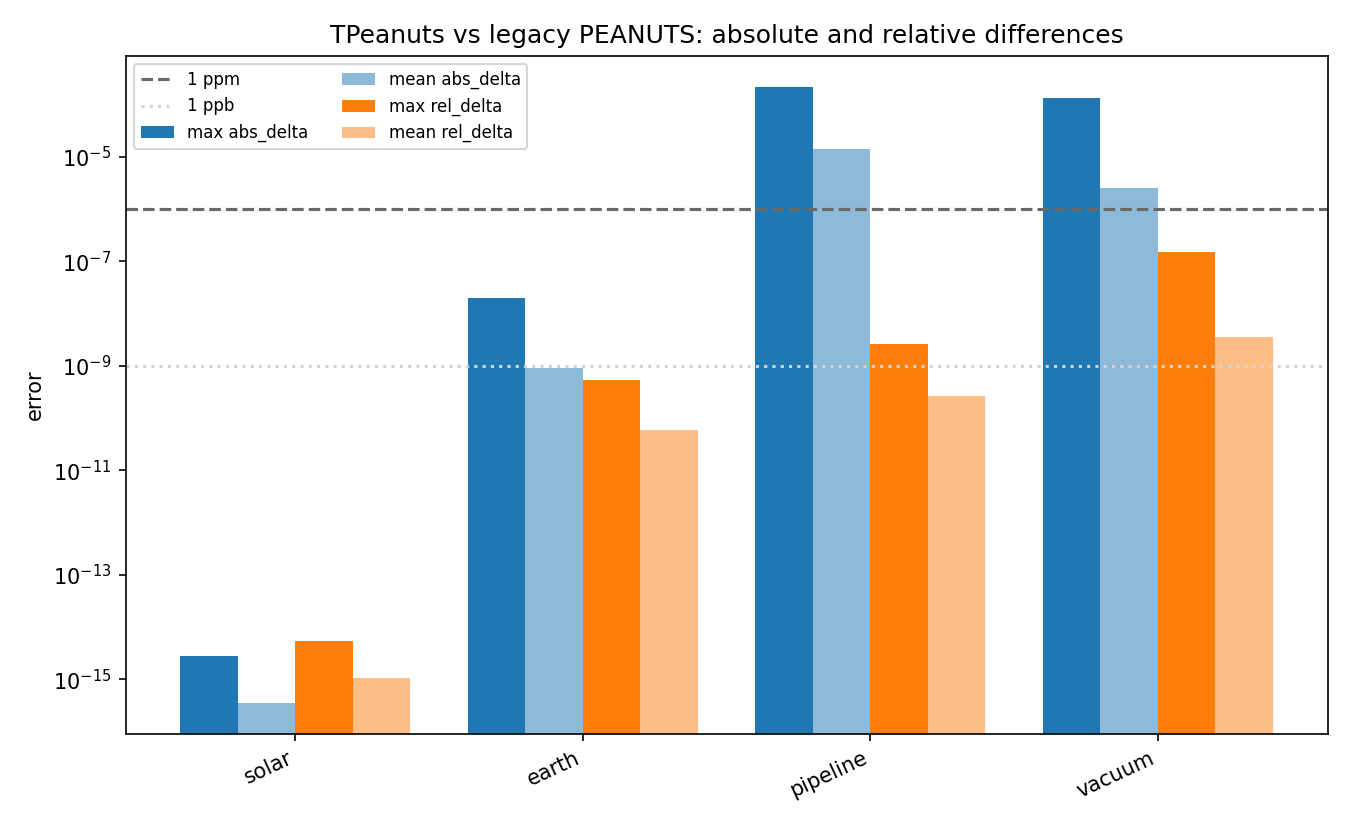
\includegraphics[width=0.528\textwidth]{figuras/resultados/validation_legacy0_summary.png}
  \hfill
  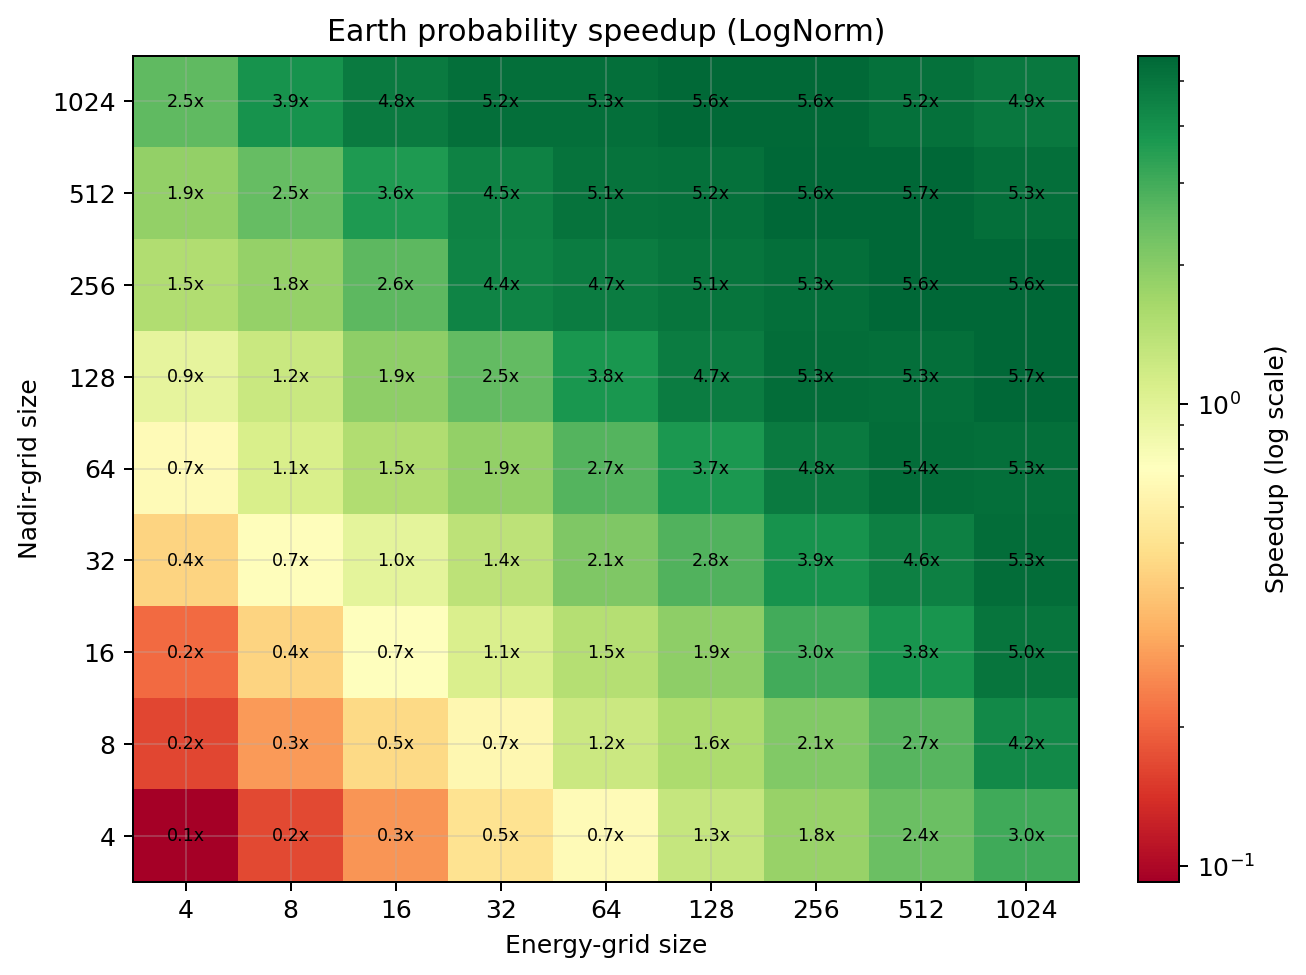
\includegraphics[width=0.432\textwidth]{figuras/resultados/earth_probability_speedup.png}
  \caption{PEANUTS validation and performance: maximum and mean absolute and relative differences between \texttt{tpeanuts} and legacy PEANUTS, by validated module, dashed and dotted lines marking the \(1\,\mathrm{ppm}\) and \(1\,\mathrm{ppb}\) reference levels (left); wall-clock speed-up of \texttt{tpeanuts} over legacy PEANUTS for the Earth-propagation probability, as a function of energy-grid and nadir-grid size (right).}
  \label{fig:peanuts-comparison}
\end{figure}

\subsubsection{nuSQuIDS validation and performance comparison}

\Cref{fig:nusquids-comparison} (left) summarises the maximum absolute and relative differences between \texttt{tpeanuts} and \texttt{nuSQuIDS} across four validated configurations: vacuum, atmosphere, solar and the composed solar-to-Earth-detection pipeline. The vacuum and atmosphere modules agree to within \(10^{-8}\)--\(10^{-7}\) in relative terms, comfortably below the \(1\,\mathrm{ppb}\) reference line, as expected for two independent, essentially exact solvers of the same closed propagation problem. The solar module and the composed solar-Earth-detection pipeline instead show markedly larger discrepancies, at the percent (\(\sim10^{-2}\)) and \(\sim10\%\) level respectively, several orders of magnitude above the vacuum/atmosphere agreement.

This pattern is consistent with the validation strategy of \cref{sec:validation-strategy}: unlike the vacuum and atmosphere cases, the solar and solar-Earth-detection observables depend on production-averaged, incoherent mass-eigenstate weights and on the treatment of coherence loss between the Sun and the Earth, both of which \texttt{tpeanuts} inherits directly from the PEANUTS convention (\cref{sec:propagation-fundamentals}) but which \texttt{nuSQuIDS} may implement through different internal approximations. The comparison against \texttt{nuSQuIDS} therefore isolates exactly the kind of convention-dependent discrepancy that a comparison against PEANUTS alone, which shares the same conventions, cannot expose.

\Cref{fig:nusquids-comparison} (right) shows the wall-clock speed-up of \texttt{tpeanuts} over \texttt{nuSQuIDS} for the integrated solar-detector probability calculation, as a function of the energy-grid and nadir/\(\cos\theta_z\)-grid sizes used in the batched evaluation. The speed-up grows monotonically with grid size, from \(\sim63\times\) for the smallest grid considered (\(2\times2\)) to over \(1100\times\) for the largest (\(32\times32\)), directly confirming the scaling behaviour anticipated in \cref{sec:validation-strategy}: because \texttt{nuSQuIDS} evaluates one solver object per energy/angle point while \texttt{tpeanuts} evaluates the full grid in a single batched call, the relative advantage of the tensor-based formulation increases with the number of configurations evaluated per call.

% TODO: notebooks/validation/nusquids/nusquids0_summary.ipynb has a prefix-mapping
% bug (PREFIX_TO_MEDIUM misses vn6_/vn7_ sterile-comparison files, producing a
% spurious 5th "unknown" bar with ~1653% error if regenerated as-is) and its
% solar/pipeline source CSVs predate the 2026-07-22/07-29 solar-physics fixes.
% Fix the mapping and re-run before regenerating the left panel below.
% TODO: the grid reported for the right panel below (2x2 to 32x32) does not
% match the grid currently defined in
% notebooks/benchmark/benchmark2_tpeanuts_vs_nusquids_performance.ipynb
% (4..256 per dimension), and no committed revision of that notebook has cached
% output for the integrated-probability cell. nuSQuIDS is not installed in the
% current environment, so these numbers cannot be regenerated or re-verified
% without a working nuSQuIDS install and a fresh, committed notebook run.
\begin{figure}[htbp]
  \centering
  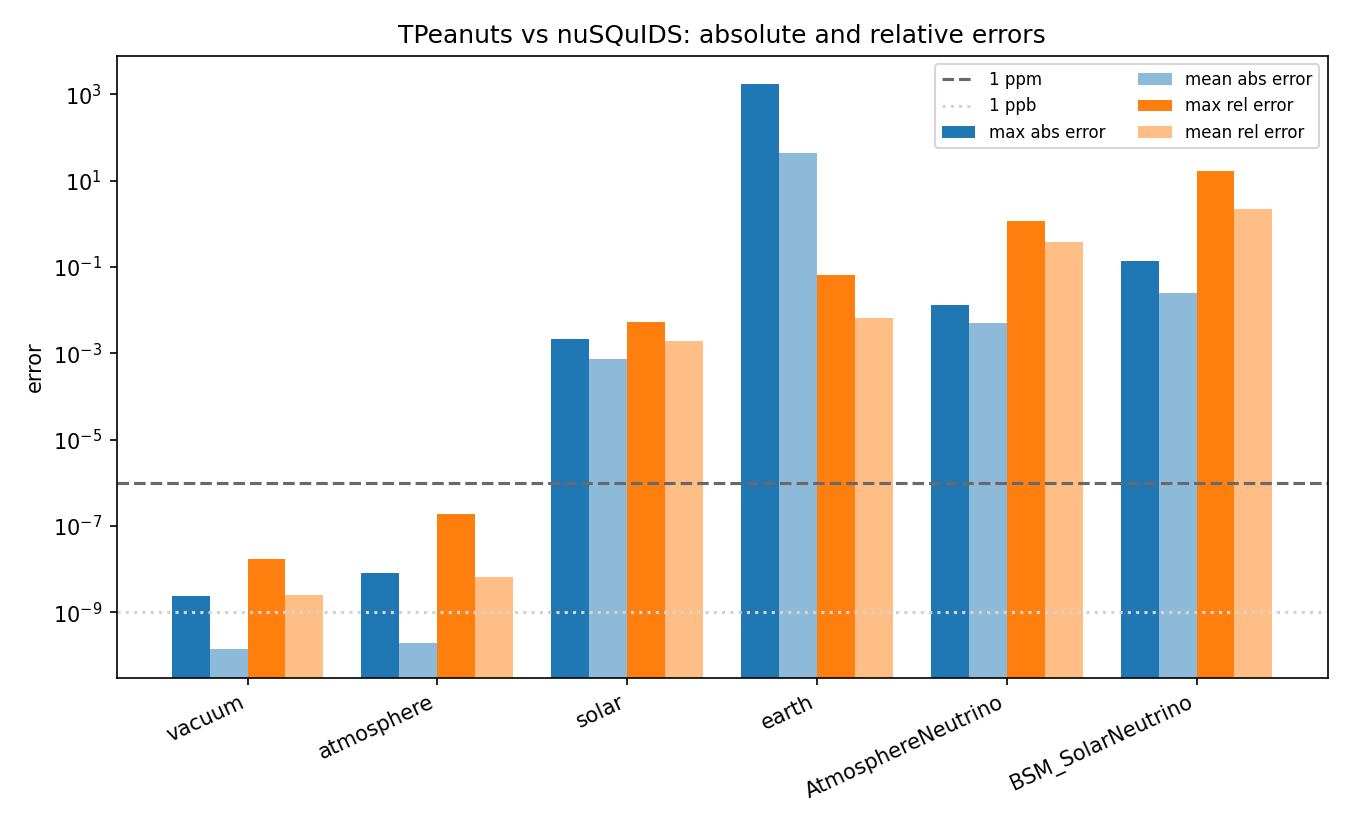
\includegraphics[width=0.530\textwidth]{figuras/resultados/vn0_summary.png}
  \hfill
  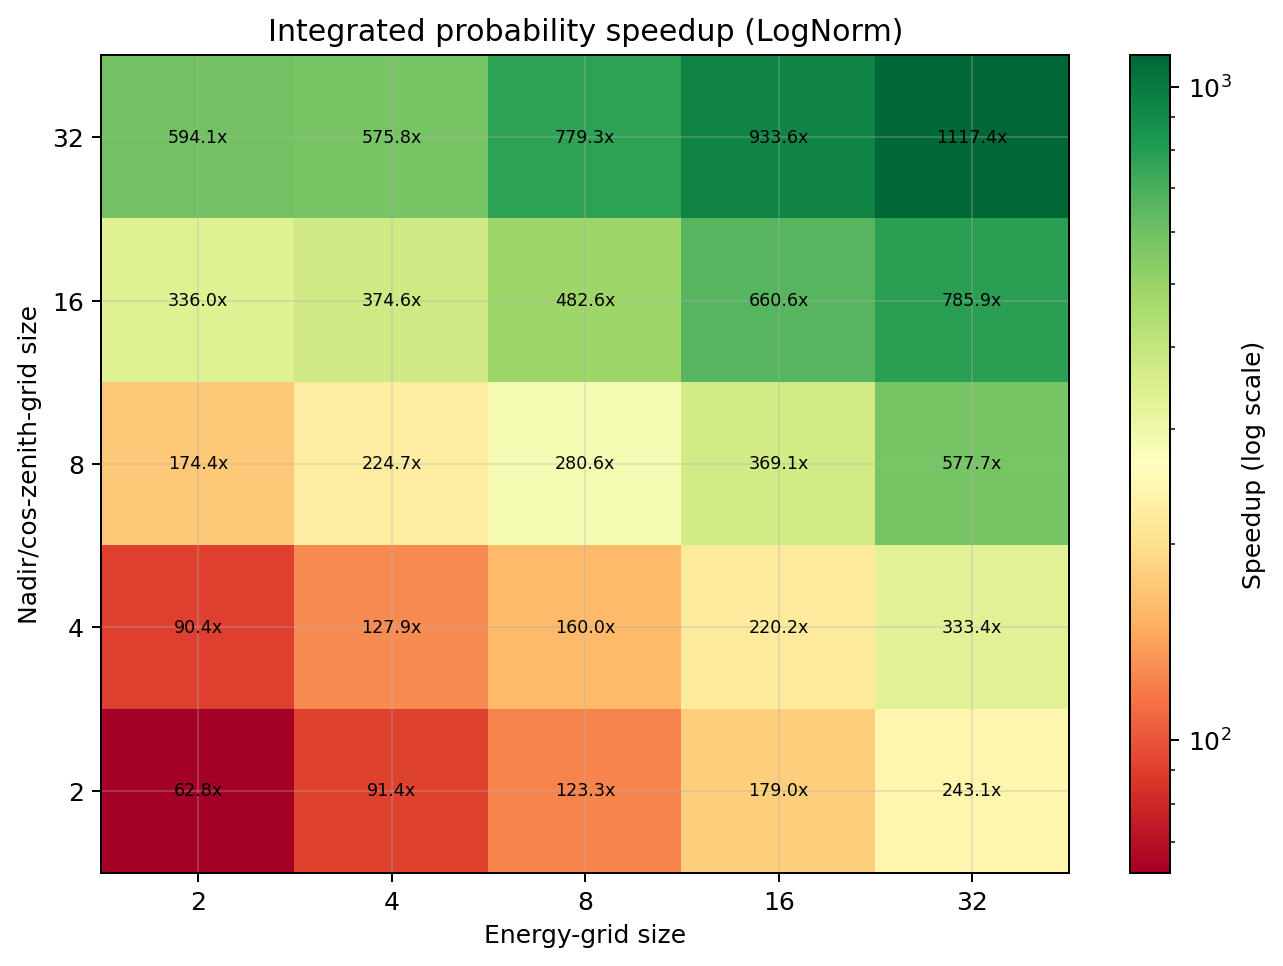
\includegraphics[width=0.430\textwidth]{figuras/resultados/integrated_probability_speedup.png}
  \caption{nuSQuIDS validation and performance: maximum and mean absolute and relative differences between \texttt{tpeanuts} and \texttt{nuSQuIDS}, by validated configuration, dashed and dotted lines marking the \(1\,\mathrm{ppm}\) and \(1\,\mathrm{ppb}\) reference levels (left); wall-clock speed-up of \texttt{tpeanuts} over \texttt{nuSQuIDS} for the integrated solar-detector probability, as a function of energy-grid and nadir-grid size (right).}
  \label{fig:nusquids-comparison}
\end{figure}

\subsection{Simulation analysis}
\label{sec:simulation-analysis-results}

Having established in \cref{sec:validation-benchmark-results} that the translated implementation is numerically reliable and computationally useful, this subsection exercises the validated engine on complete vacuum, solar- and atmospheric-neutrino propagation pipelines, from production through Earth regeneration, rather than a single isolated probability, checking each result against the qualitative or quantitative behaviour expected from the standard oscillation phenomenology. \Cref{sec:experimental-reproduction-results} then goes further, reproducing a series of specific, well-known experimental signatures with the same engine.

\subsubsection{Vacuum neutrino}

\Cref{fig:vacuum-2d-maps} maps the vacuum survival probability \(P(\nu_e\to\nu_e)\) and the vacuum appearance probability \(P(\nu_\mu\to\nu_e)\) over the full \((L,E)\) plane, \(L\) from \(1\) to \(1.5\times10^4\,\mathrm{km}\) and \(E\) from \(0.1\) to \(10\,\mathrm{GeV}\), the baseline/energy range spanning reactor, accelerator and atmospheric configurations within a single, common map. Both channels are governed by the same oscillatory phase \(1.267\,\Delta m^2_{31}L/E\), so the diagonal fringes of \(P_{ee}\) and \(P_{\mu e}\) run parallel and are exactly complementary at leading order: \(P_{ee}\) is close to unity (light) wherever \(P_{\mu e}\) is close to zero (light), and \(P_{ee}\) dips towards its first oscillation minimum (dark blue) exactly where \(P_{\mu e}\) peaks near its maximum appearance amplitude (dark, \(\sim0.15\)), consistent with two-flavour-dominated conversion at fixed \(L/E\) once the sub-leading solar splitting is neglected. The fine chequerboard structure visible at the largest \(L/E\), most pronounced in the bottom-right corner of both panels, is the beat pattern between the atmospheric and solar mass splittings rather than numerical noise: at those baselines and energies the solar phase \(\Delta m^2_{21}L/E\) has itself completed many cycles, so the combined pattern aliases against the finite grid resolution used to render the map. Every pixel is computed from the full three-flavour vacuum evolution operator, so this map is a single, direct consistency check that the implementation reproduces the correct \(L/E\) scaling and relative amplitude of survival and appearance before any matter effect is introduced, complementing the CP-violation check of \cref{fig:cp-asymmetry-dune} below, which isolates the phase structure of the same vacuum evolution operator rather than its \(L/E\) scaling.

\begin{figure}[htbp]
  \centering
  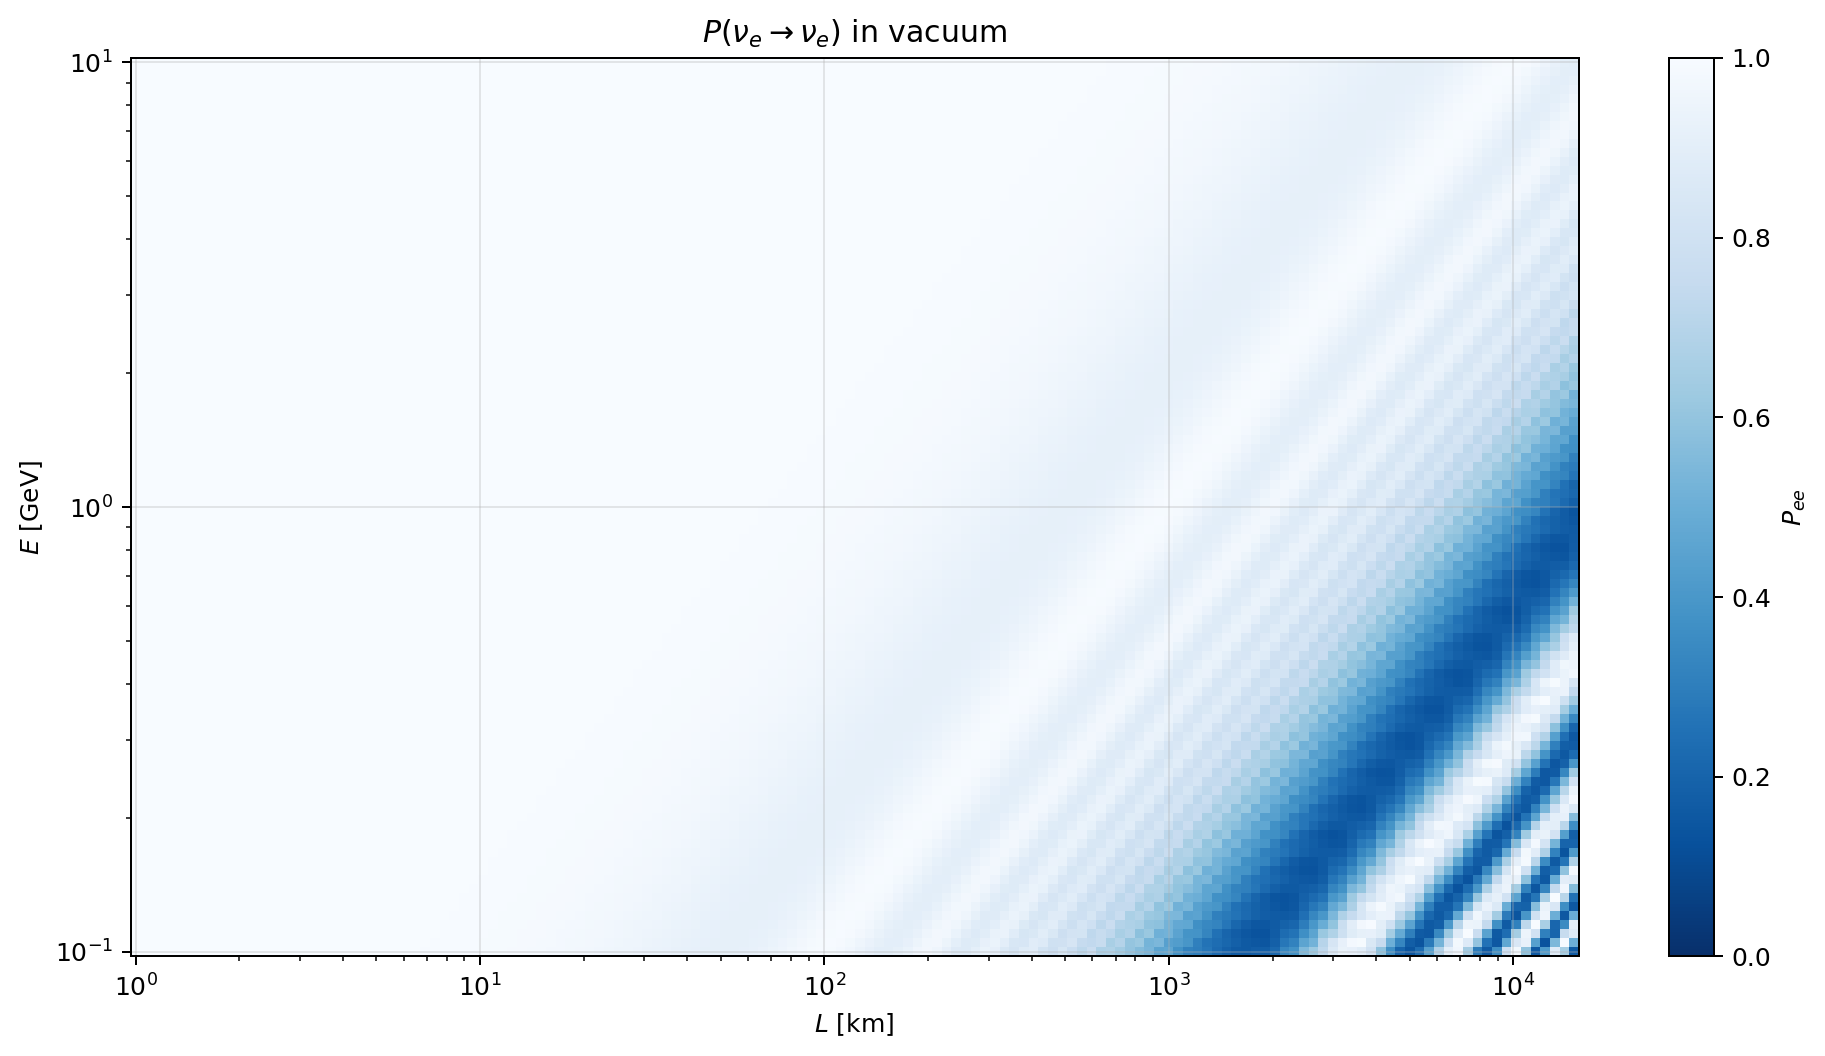
\includegraphics[width=0.48\textwidth]{figuras/resultados/vf1_fig61_1_pee_2d_map.png}
  \hfill
  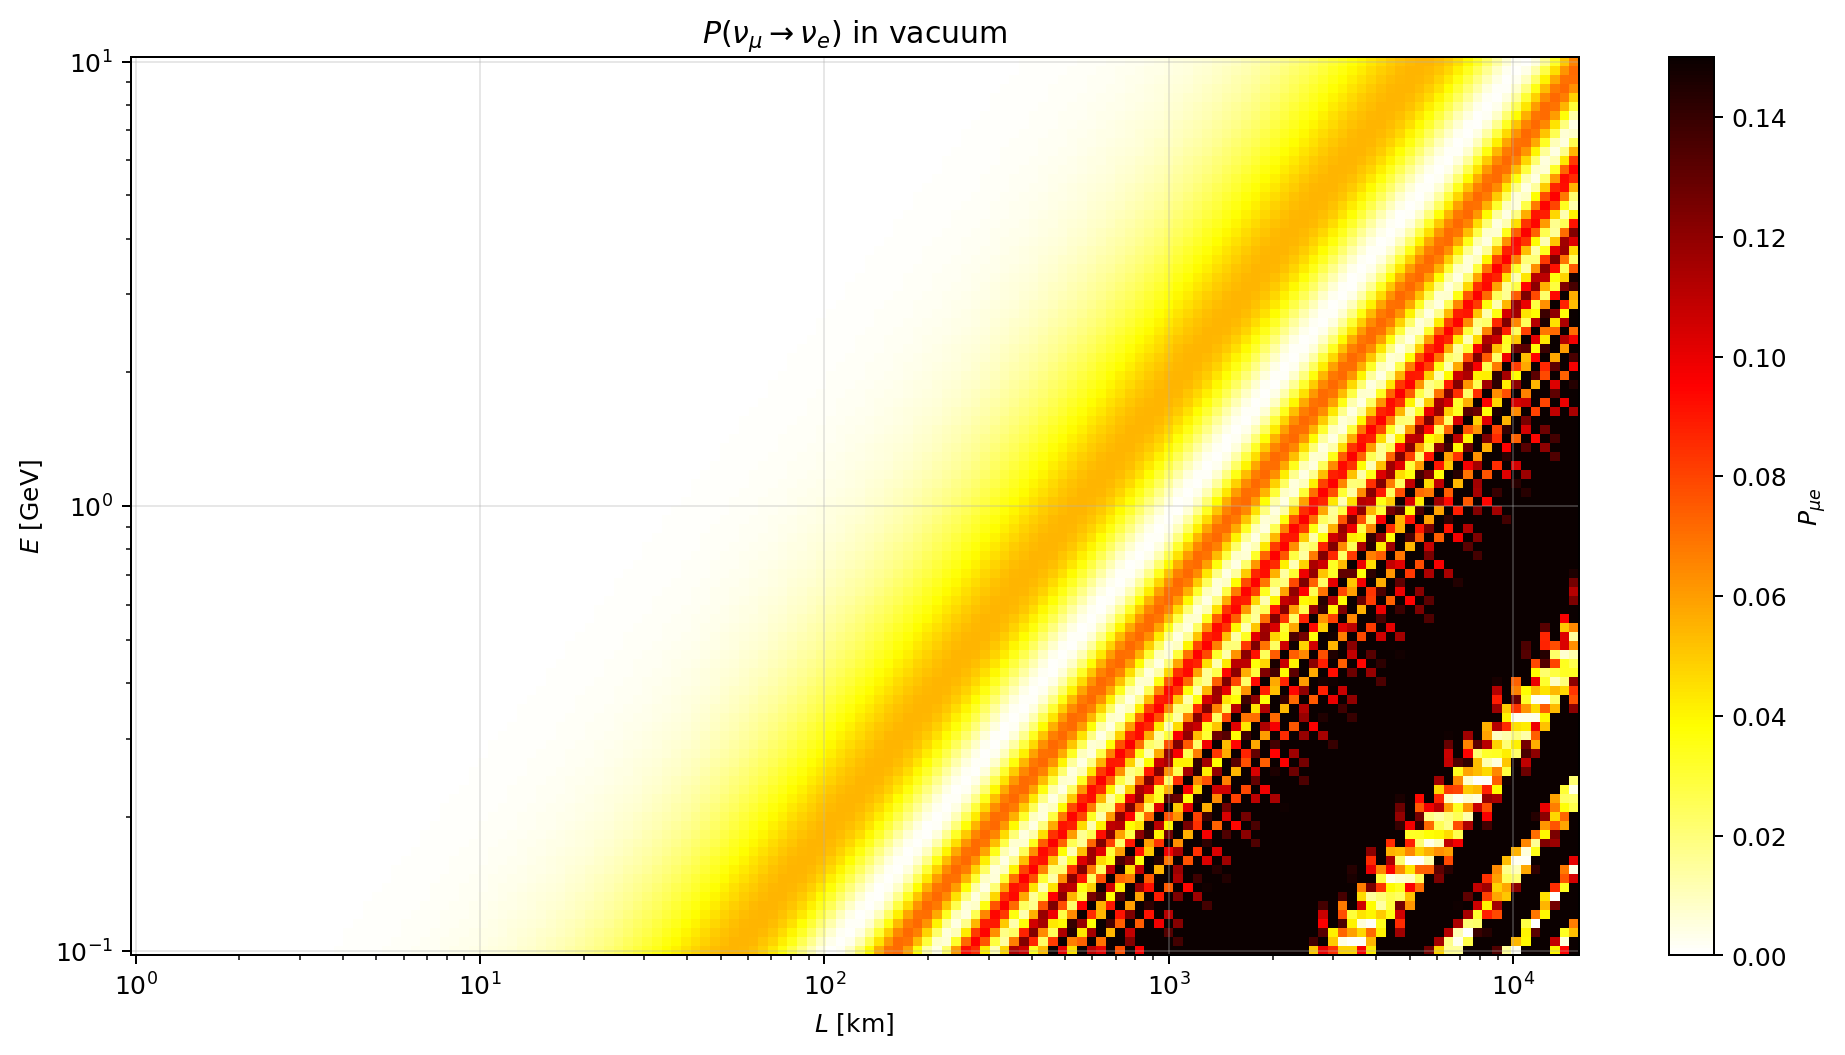
\includegraphics[width=0.48\textwidth]{figuras/resultados/vf1_fig62_1_pemu_2d_map.png}
  \caption{Vacuum oscillation probabilities over the \((L,E)\) plane: survival \(P(\nu_e\to\nu_e)\) (left) and appearance \(P(\nu_\mu\to\nu_e)\) (right).}
  \label{fig:vacuum-2d-maps}
\end{figure}

\subsubsection{Solar neutrino}

\Cref{fig:solar-earth-regeneration} shows the Earth-regeneration probability \(P(\nu_\odot\to\nu_\alpha;E)\) for incoherent solar \(^8\mathrm{B}\) mass-basis weights propagated along four representative nadir-angle trajectories, crossing the inner core, outer core, mantle and crust only, against the no-Earth vacuum reference. Below \(\sim4\,\mathrm{MeV}\) every trajectory overlaps the vacuum curve almost exactly, since the day--night regeneration mechanism scales with the matter path length and electron density integrated along the trajectory, both small compared with the vacuum oscillation length at these energies. Above \(\sim6\,\mathrm{MeV}\) the curves separate visibly from vacuum and from each other, with the inner-core-crossing trajectory showing the largest departure, consistent with its longer, denser matter path driving the strongest regeneration, the same mechanism quantified through the day--night asymmetry in \cref{sec:solar-day-night} below. The three flavour channels remain unitary at every energy and trajectory, \(\sum_\alpha P(\nu_\odot\to\nu_\alpha)=1\), confirming that Earth regeneration redistributes flavour content without any leakage.

\begin{figure}[htbp]
  \centering
  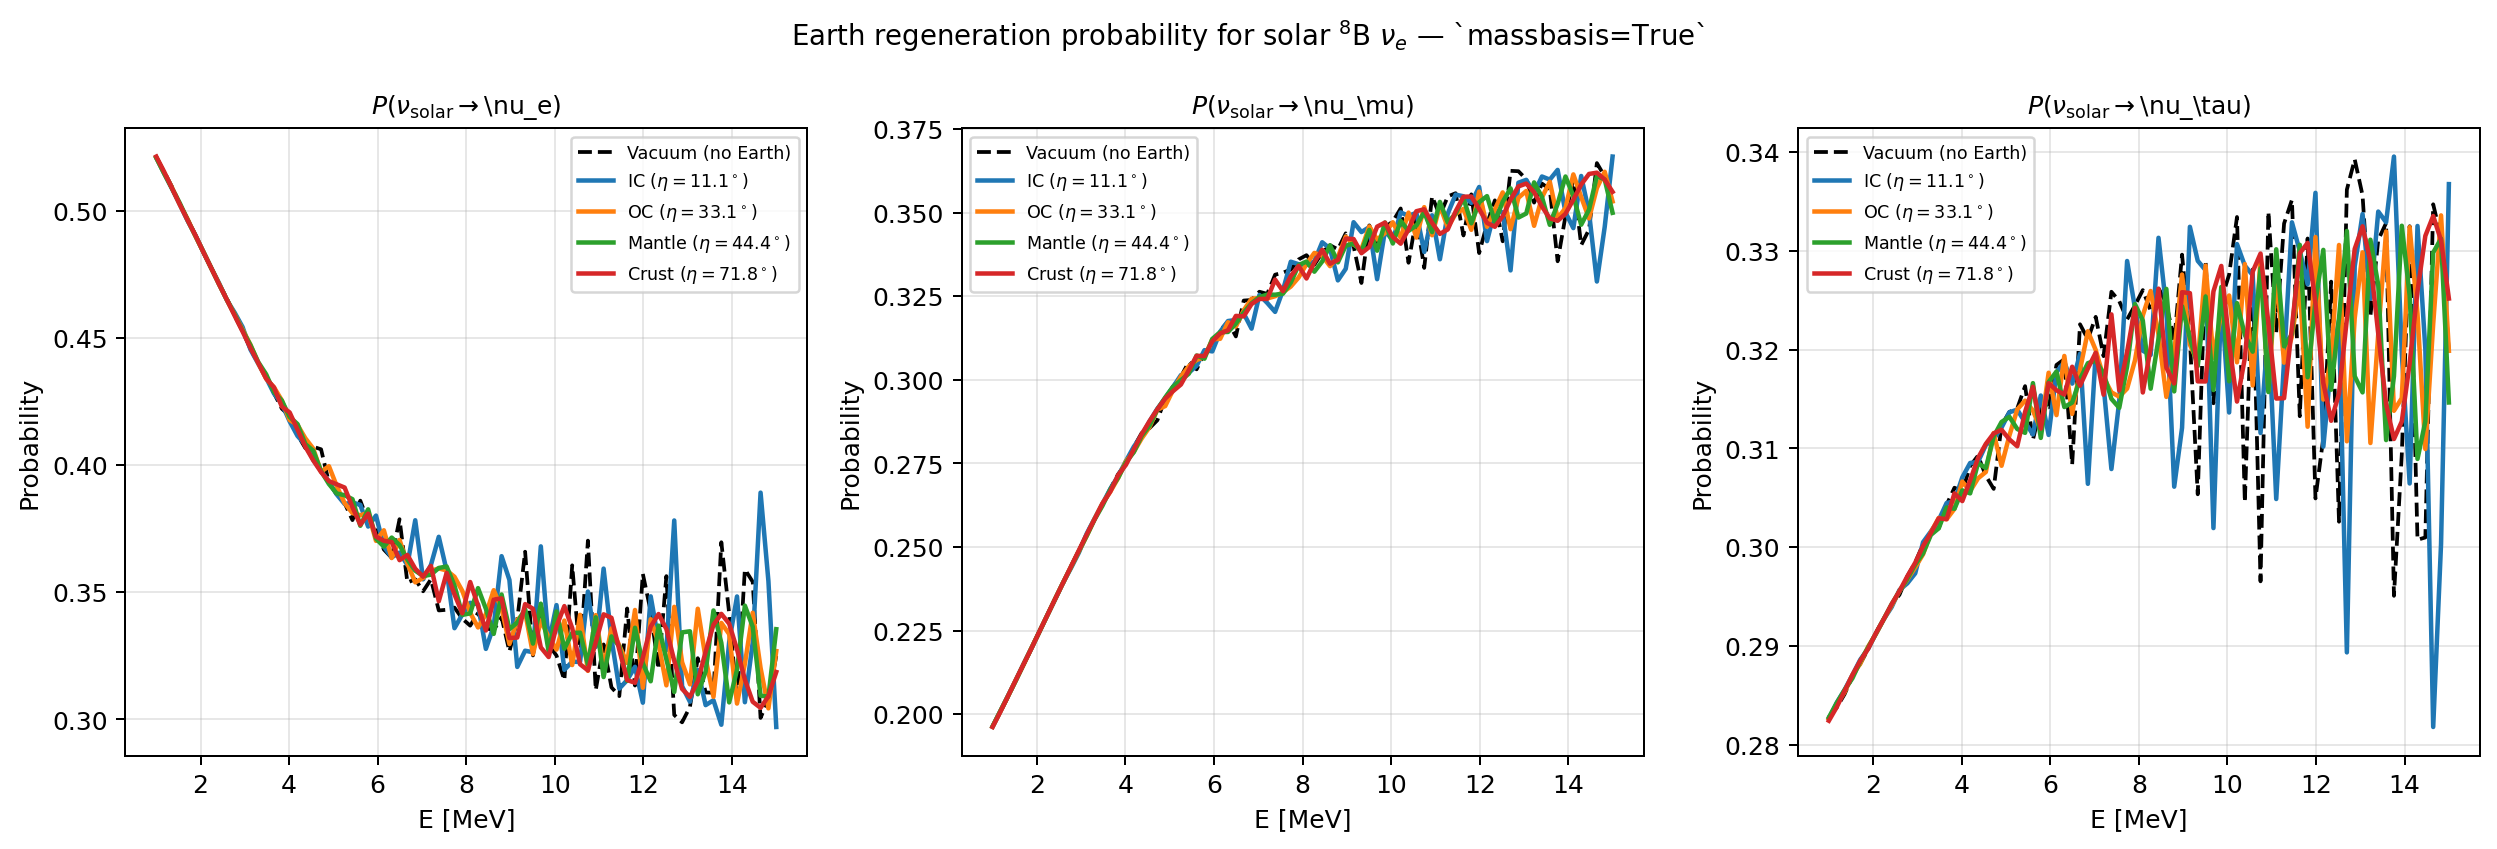
\includegraphics[width=\textwidth]{figuras/resultados/ef3_fig41_pearth_solar.png}
  \caption{Earth-regeneration probability for solar \(^8\mathrm{B}\) neutrinos produced as incoherent mass-basis weights, \(P(\nu_\odot\to\nu_\alpha;E)\), for four representative nadir-angle trajectories crossing the inner core, outer core, mantle and crust, compared with the no-Earth vacuum reference.}
  \label{fig:solar-earth-regeneration}
\end{figure}

\Cref{fig:solar-total-flux} exercises the solar propagation pipeline with all solar production channels combined (\(pp\), \(pep\), \(hep\), \({}^7\mathrm{Be}\), \({}^8\mathrm{B}\), \({}^{13}\mathrm{N}\), \({}^{15}\mathrm{O}\), \({}^{17}\mathrm{F}\)), giving the total flavour flux \(\Phi_\alpha^{\mathrm{tot}}(E,\eta_{\mathrm{fix}})\) reaching the Earth's surface at a fixed nadir angle. The \(\nu_e\) flux falls steadily from \(\sim3.5\times10^{10}\) to \(\sim2\times10^{10}\,\mathrm{cm^{-2}\,s^{-1}}\) as the survival probability decreases with energy, while \(\nu_\mu\) and \(\nu_\tau\) grow correspondingly and converge above \(\sim9\,\mathrm{MeV}\), consistent with the near-equal \(\mu\)/\(\tau\) appearance implied by the PMNS structure in the solar sector.

\begin{figure}[htbp]
  \centering
  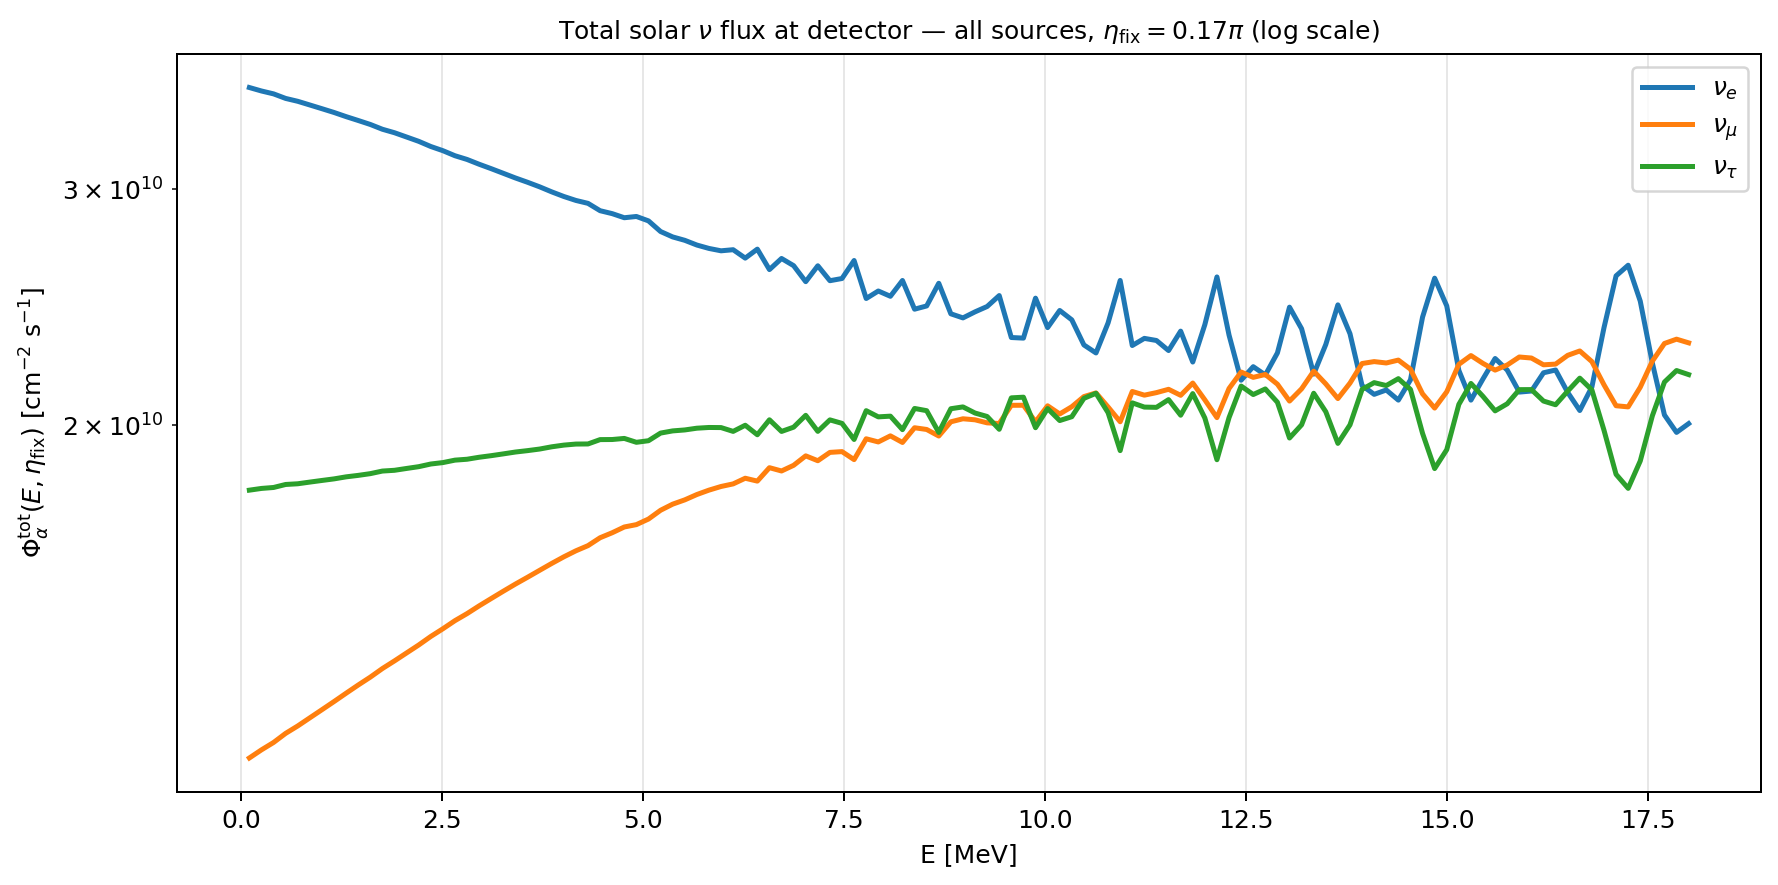
\includegraphics[width=0.85\textwidth]{figuras/resultados/ef3_fig51_flux_total_spectrum.png}
  \caption{Total solar-neutrino flux reaching the Earth's surface, \(\Phi_\alpha^{\mathrm{tot}}(E,\eta_{\mathrm{fix}})\), summed over all solar production channels, at fixed nadir angle \(\eta_{\mathrm{fix}}=0.17\pi\).}
  \label{fig:solar-total-flux}
\end{figure}

Isolating the \({}^8\mathrm{B}\) channel and exercising the nadir-angle exposure integration for four representative surface latitudes gives three flavour spectra that are, to the resolution of the plot, indistinguishable across all four: annual averaging over the day/night nadir-angle exposure smooths out the latitude-dependent matter effects seen in \cref{fig:solar-total-flux}, as expected from the small latitude differences considered.

\subsubsection{Atmospheric neutrino}

The atmospheric detection pipeline (\cref{sec:pipelines}) requires, as a boundary condition, the production-height distribution of the parent flux at each energy and angle. \Cref{fig:atm-production-height} compares this distribution, \(f(h|E,\alpha)\), for \(\nu_\mu\) at a fixed zenith angle (\(\alpha=31.8^\circ\)) as generated by MCEq \parencite{Fedynitch2015} and by the tabulated Honda/HKKM parametrisation \parencite{Honda2007}. Both place the bulk of the production between \(\sim10\) and \(30\,\mathrm{km}\), peaking around \(15\,\mathrm{km}\) and shifting slightly higher at higher energy; the visibly discretised Honda distribution reflects its coarser production-height binning, but the two agree closely in shape and normalisation.

\begin{figure}[htbp]
  \centering
  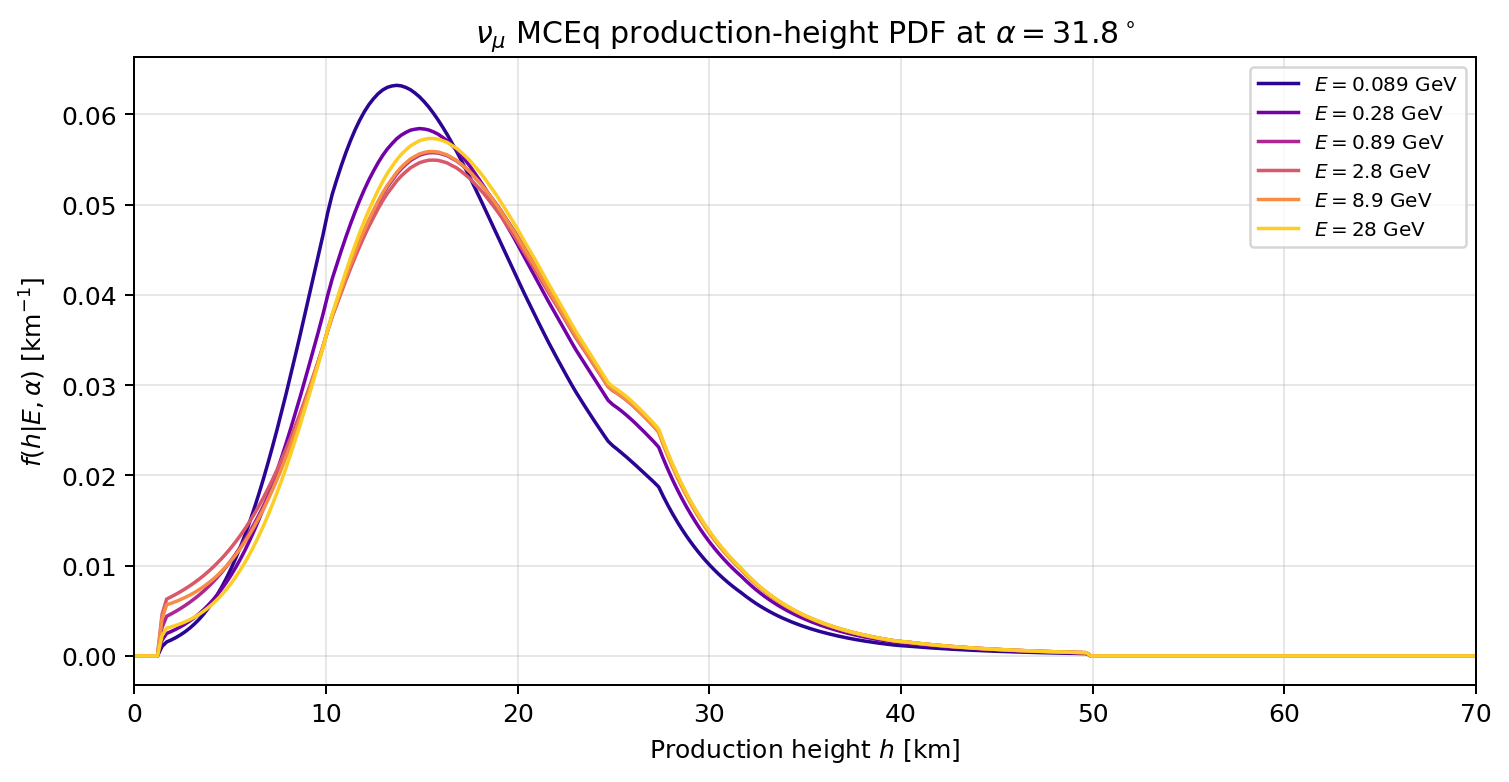
\includegraphics[width=0.48\textwidth]{figuras/resultados/atm5_fig64_fEh.png}
  \hfill
  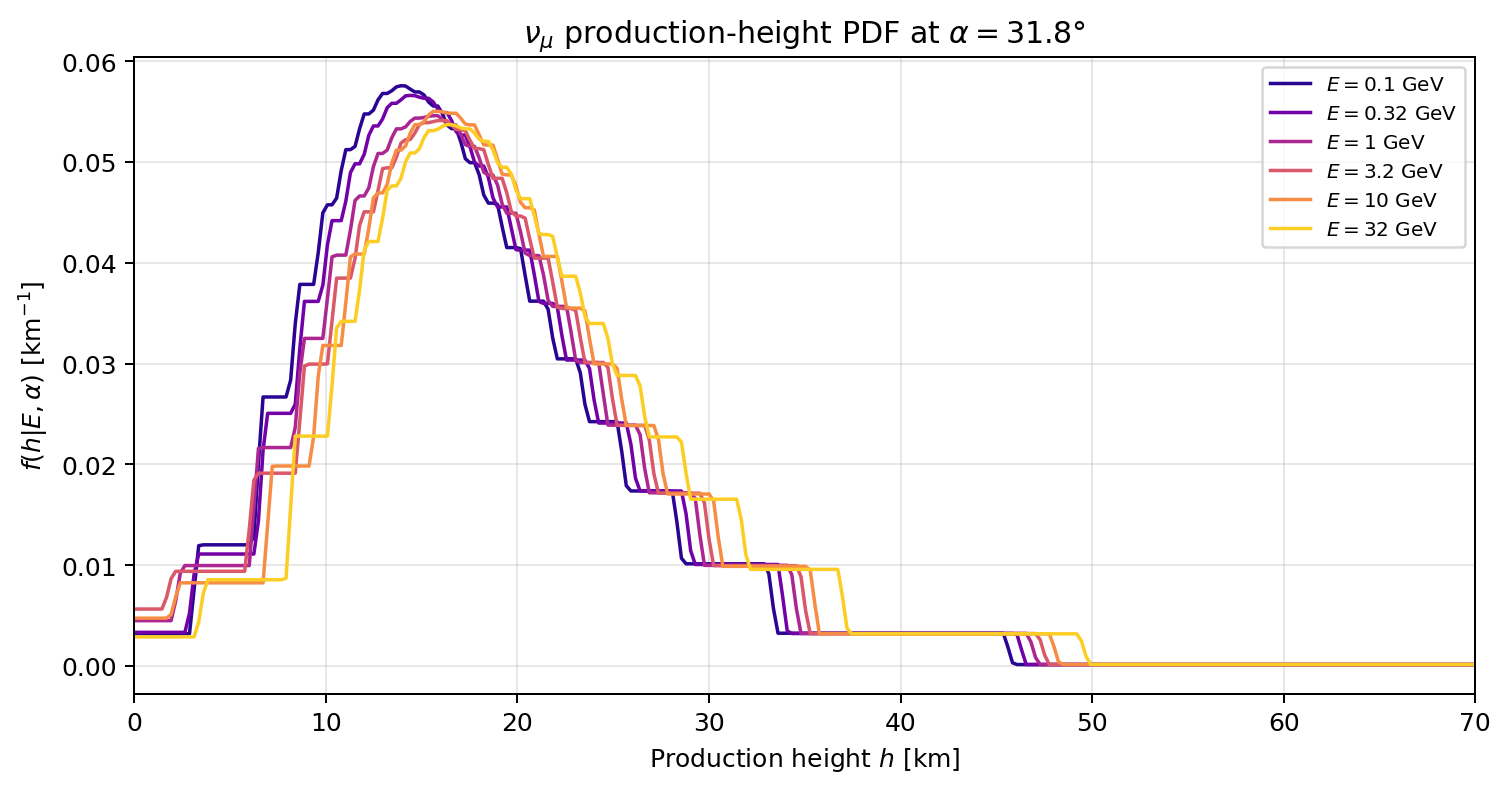
\includegraphics[width=0.48\textwidth]{figuras/resultados/atm3_fig64_fEh_honda.png}
  \caption{\(\nu_\mu\) production-height probability density, \(f(h|E,\alpha)\), at fixed zenith angle \(\alpha=31.8^\circ\), generated with MCEq (left) \parencite{Fedynitch2015} and with the Honda/HKKM parametrisation (right) \parencite{Honda2007}.}
  \label{fig:atm-production-height}
\end{figure}

\Cref{fig:atm-surface-probability} shows the corresponding surface oscillation probabilities \(P(\bar\nu_\mu\to\bar\nu_\alpha;E,h)\) for an antimuon-neutrino primary at fixed zenith angle \(\theta=18.2^\circ\), as a function of energy and production height, before folding in the production-height distribution of \cref{fig:atm-production-height} or propagating further through the Earth. Survival dominates almost everywhere above \(\sim0.3\,\mathrm{GeV}\), \(P(\bar\nu_\mu\to\bar\nu_\mu)\gtrsim0.8\), while the appearance channels \(P(\bar\nu_\mu\to\bar\nu_e)\) and \(P(\bar\nu_\mu\to\bar\nu_\tau)\) are confined to a narrow band below \(\sim0.3\,\mathrm{GeV}\) that widens with production height, tracing out the longer atmospheric path length available to neutrinos produced higher up, exactly the \(L/E\)-driven onset of oscillation expected before any Earth matter effect is introduced.

\begin{figure}[htbp]
  \centering
  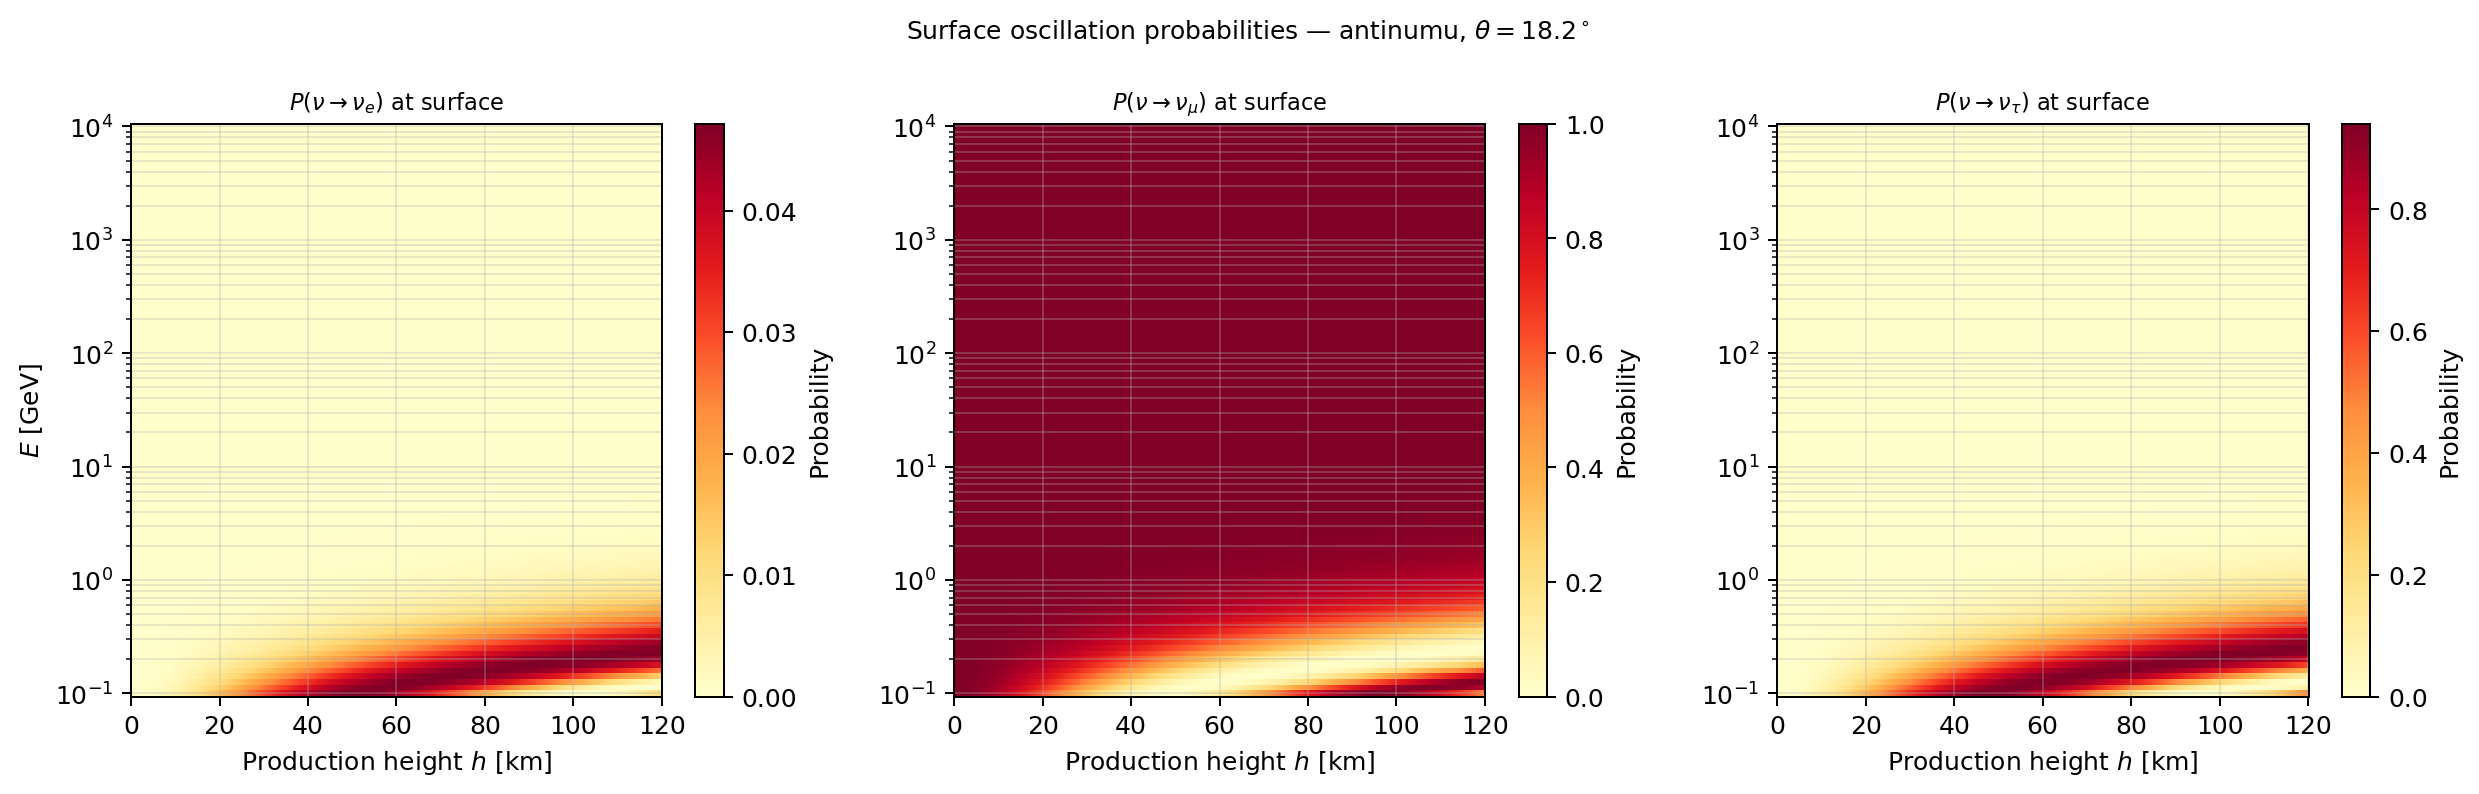
\includegraphics[width=\textwidth]{figuras/resultados/atm6_fig41_surface_prob.png}
  \caption{Surface oscillation probabilities \(P(\bar\nu_\mu\to\bar\nu_\alpha;E,h)\) for an antimuon-neutrino primary at fixed zenith angle \(\theta=18.2^\circ\), as a function of energy and production height.}
  \label{fig:atm-surface-probability}
\end{figure}

\Cref{fig:atm-survival-heatmap} shows the resulting detector-level \(\nu_\mu\) survival probability, \(P_{\mathrm{det}}(\nu_\mu\to\nu_\mu;E,\theta)\), after propagation through the atmosphere and Earth and averaging over the production-height distribution of \cref{fig:atm-production-height}. The pipeline reproduces the expected atmospheric \(\nu_\mu\) disappearance: survival close to unity at high energy (\(E\gtrsim100\,\mathrm{GeV}\)), decreasing towards \(\sim0.1\text{--}0.2\) at sub-GeV energies and large zenith angles, confirming that the height-integration and flavour-summation stages combine correctly with the oscillation engine.

\begin{figure}[htbp]
  \centering
  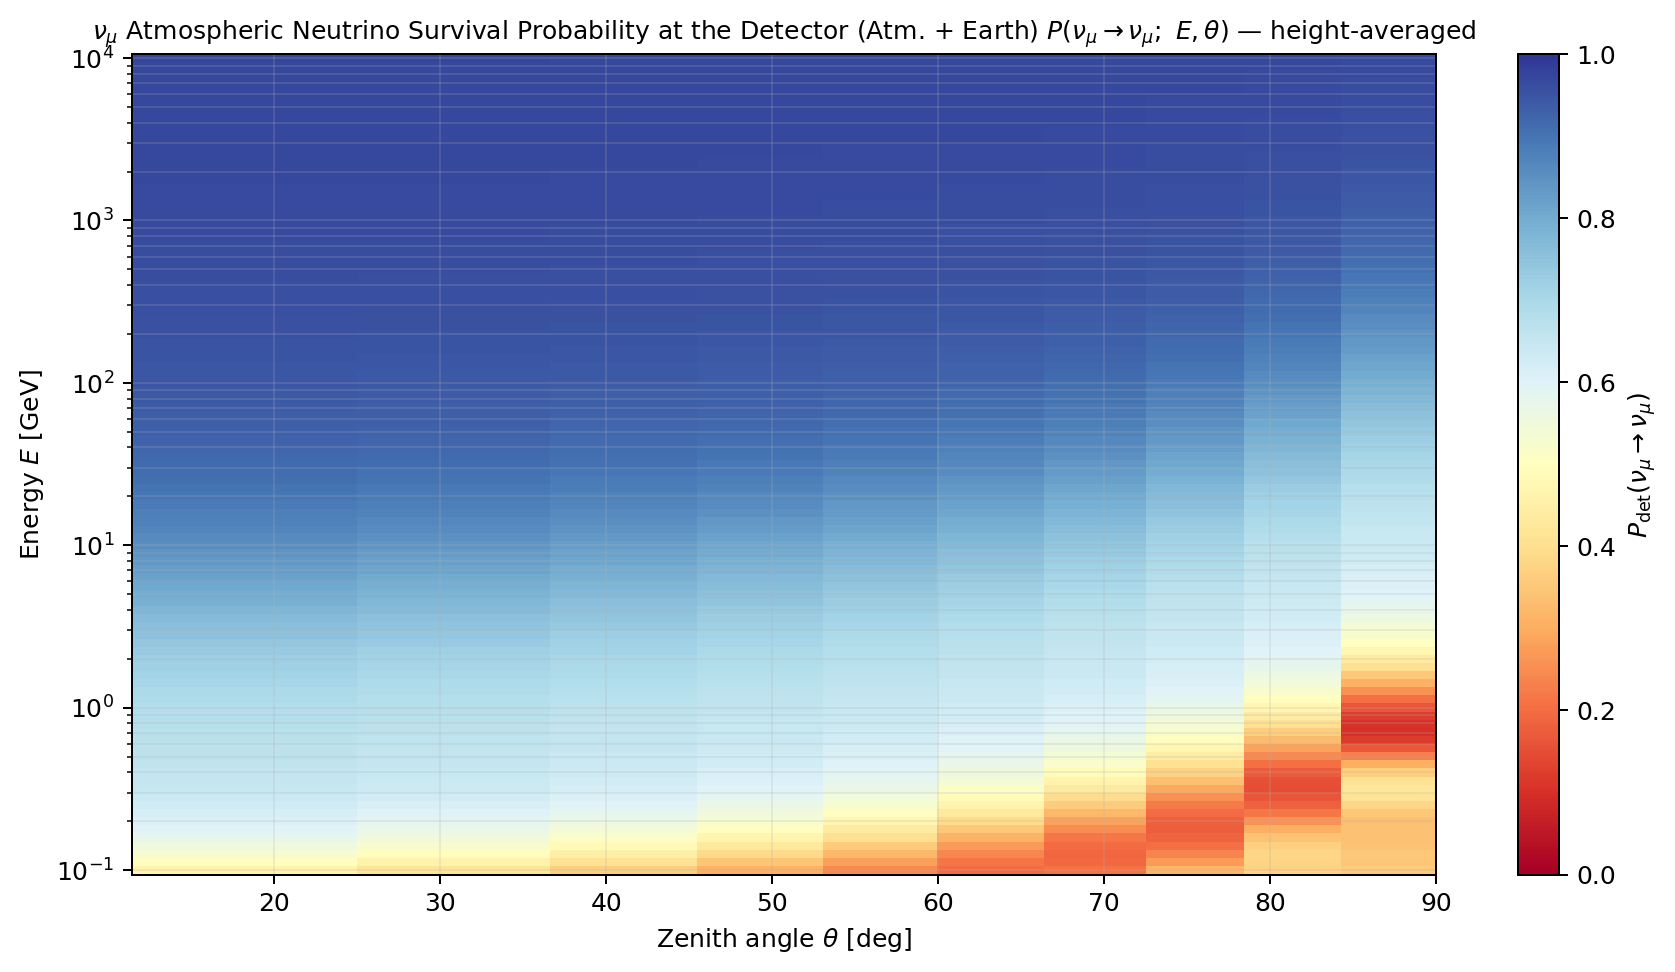
\includegraphics[width=0.8\textwidth]{figuras/resultados/atm6_fig63_prob_heatmap.png}
  \caption{Height-averaged, detector-level \(\nu_\mu\) survival probability \(P_{\mathrm{det}}(\nu_\mu\to\nu_\mu;E,\theta)\), combining atmospheric and Earth propagation.}
  \label{fig:atm-survival-heatmap}
\end{figure}

\subsection{Reproduction of experimental results}
\label{sec:experimental-reproduction-results}

Building on the validated propagation pipelines of \cref{sec:simulation-analysis-results}, this subsection reproduces a series of specific, well-known experimental and phenomenological signatures, the solar day--night asymmetry, the MSW resonance and the adiabatic limit it relies on, CP violation, atmospheric oscillograms, and Earth matter tomography, each checked against a published measurement or an analytic expectation rather than only a qualitative pattern.

\subsubsection{Solar day--night asymmetry}
\label{sec:solar-day-night}

The regeneration of solar \(\nu_e\) inside the Earth during night-time observation is quantified by the day--night asymmetry \(A_{\mathrm{DN}}=2(P_{ee}^{\mathrm{day}}-P_{ee}^{\mathrm{night}})/(P_{ee}^{\mathrm{day}}+P_{ee}^{\mathrm{night}})\), computed here for the \({}^8\mathrm{B}\) flux using the NuFIT~5.2 normal-ordering parameters \parencite{NuFit52}. The flux-weighted, energy-integrated asymmetry \(A_{\mathrm{DN}}^{\mathrm{int}}\), obtained for four representative detector sites (Super-K, Borexino, SNO+, JUNO), is compared directly against the Super-Kamiokande-IV measurement: all four predictions, \(-2.6\%\) to \(-2.85\%\), fall within the experimental \(1\sigma\) band, \((-3.2\pm1.2)\%\) \parencite{SuperKamiokande2016}, confirming that the solar detection pipeline reproduces the observed regeneration signal within present experimental precision.

A more detailed, detector-specific comparison additionally accounts for two effects relevant to the Super-Kamiokande measurement: its \(3.5\,\mathrm{MeV}\) electron-recoil cut corresponds to a higher effective neutrino-energy threshold, \(E_\nu^{\mathrm{eff}}\approx5.5\,\mathrm{MeV}\), and the observed rate is weighted by the full elastic-scattering cross section rather than by the neutrino spectrum alone. \Cref{tab:solar-dn-comparison} shows that both corrections push the predicted asymmetry closer to the measured value at every site, from \(-2.69\%\) to \(-3.20\%\) at Super-K, in better agreement with the SK-IV measurement and consistent with the mild (\(\sim1.3\sigma\)) tension already present between that measurement and the independent LMA-MSW theoretical range.

\begin{table}[htbp]
  \centering
  \footnotesize
  \caption{Day--night asymmetry \(A_{\mathrm{DN}}^{\mathrm{int}}\) at each detector site: as computed (\(E_\nu>3.5\,\mathrm{MeV}\) threshold, spectral weight only) and with the two Super-Kamiokande-specific corrections applied, compared against the independent LMA-MSW prediction and the Super-Kamiokande-IV measurement (Super-K only).}
  \label{tab:solar-dn-comparison}
  \begin{tabular}{@{}lrrrr@{}}
    \toprule
    Detector & \texttt{tpeanuts} & \texttt{tpeanuts-sk} & LMA std. & Published \\
    \midrule
    Super-K  & \(-2.69\%\) & \(-3.20\%\) & \(-2.0\%\) to \(-1.7\%\) & \((-3.2\pm1.2)\%\) \\
    Borexino & \(-2.76\%\) & \(-3.27\%\) & --- & --- \\
    SNO+     & \(-2.83\%\) & \(-3.33\%\) & --- & --- \\
    JUNO     & \(-2.59\%\) & \(-3.10\%\) & --- & --- \\
    \bottomrule
  \end{tabular}
\end{table}

\subsubsection{MSW resonance}

The MSW resonance condition, \(V_k(\rho)=\cos2\theta_{12}\), is located along the solar density profile for several neutrino energies. At low energy (\(E\lesssim1.5\,\mathrm{MeV}\)) the potential never reaches the resonance condition within the Sun, so \(pp\)-like neutrinos propagate quasi-adiabatically without crossing resonance; as the energy increases, the resonance radius \(\rho_{\mathrm{res}}\) moves outward, from \(\rho_{\mathrm{res}}=0.032\) at \(2\,\mathrm{MeV}\) to \(\rho_{\mathrm{res}}=0.282\) at \(15\,\mathrm{MeV}\), reproducing the expected energy dependence of the MSW resonance layer. \Cref{fig:msw-local-pee} shows the local survival probability \(P_{ee}(\rho,E)\) across the production region. At low energy, \(P_{ee}\) remains close to the vacuum-averaged value, \(\sum_i|U_{ei}|^4=0.553\), throughout the Sun; at high energy, \(P_{ee}\) starts near the adiabatic matter-eigenstate limit, \(|U_{e2}|^2=0.296\), at the production point and relaxes smoothly to the vacuum-averaged value as the neutrino exits the Sun, exactly as expected from adiabatic MSW conversion.

\begin{figure}[htbp]
  \centering
  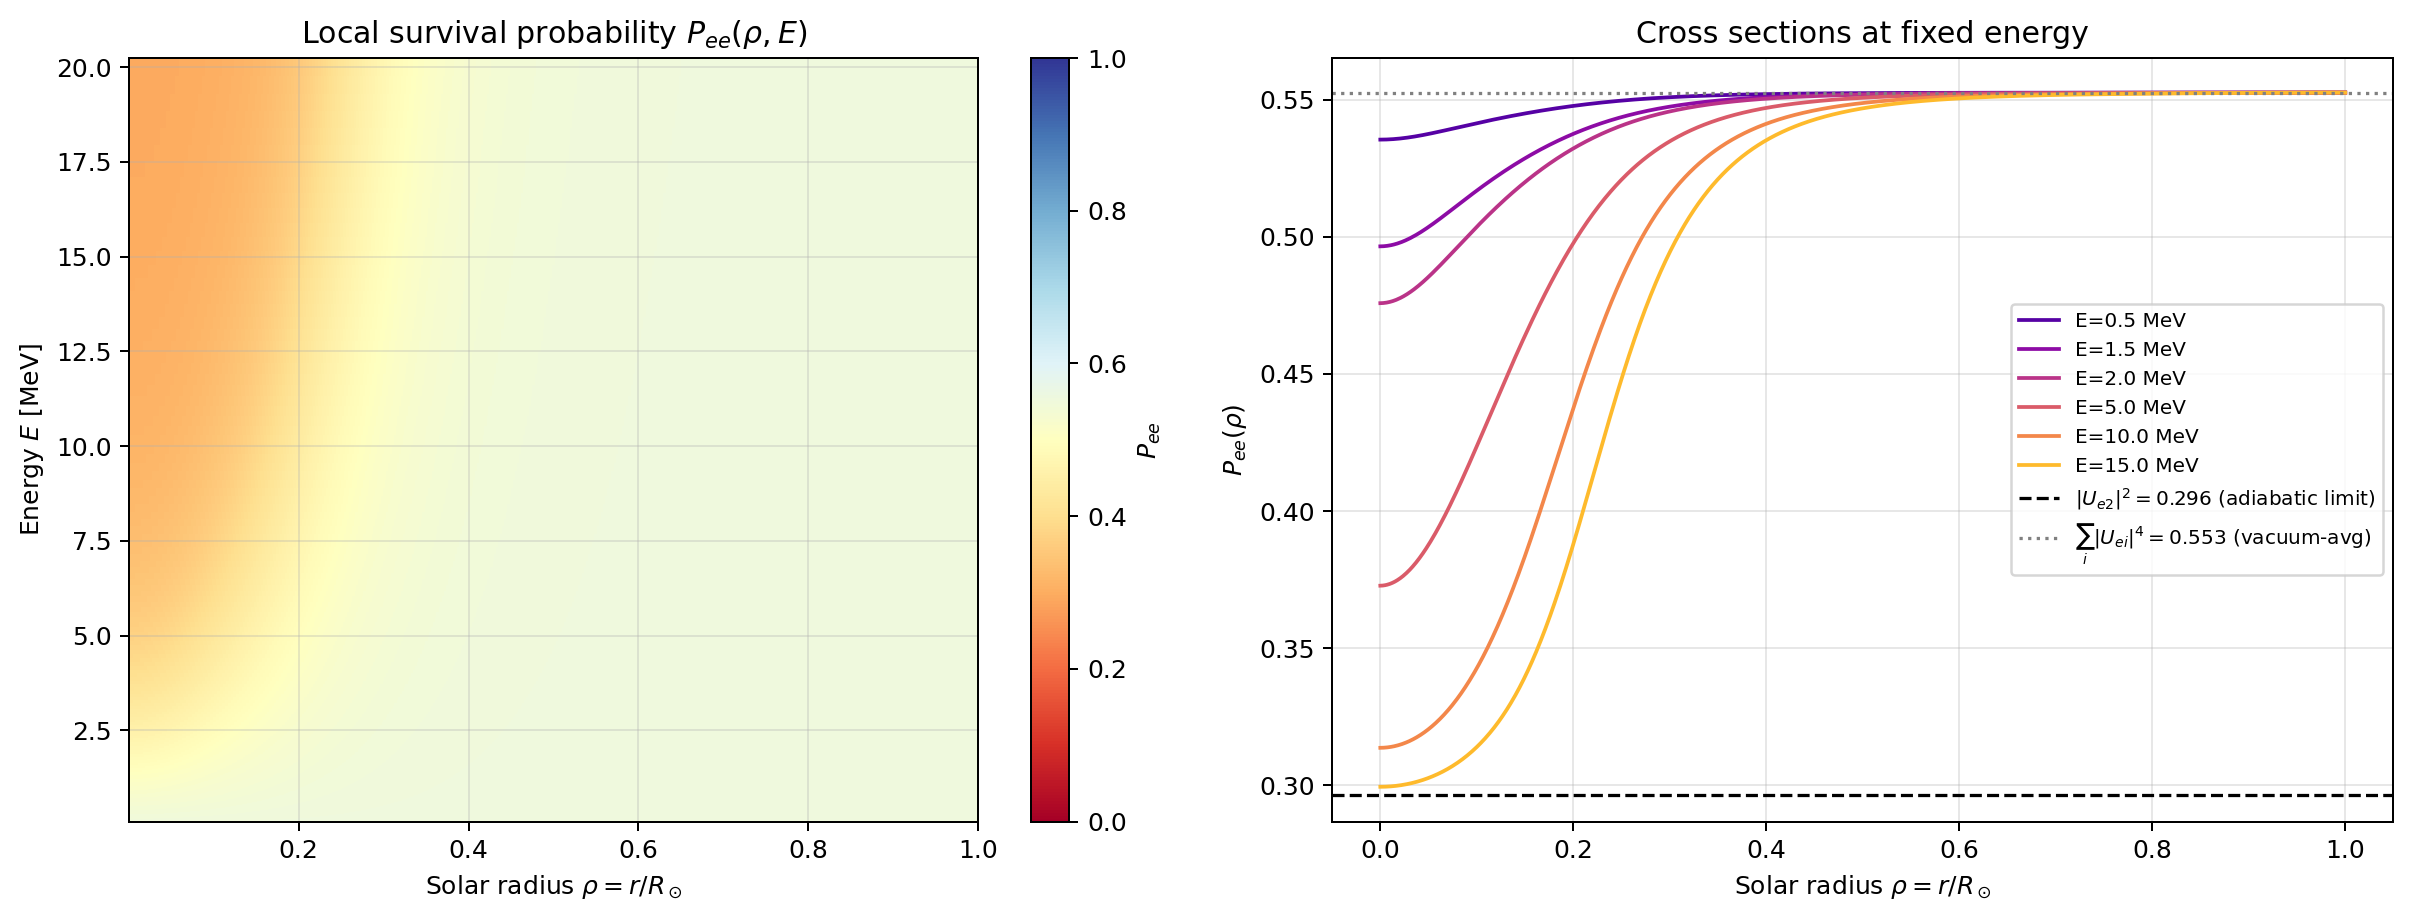
\includegraphics[width=\textwidth]{figuras/resultados/sn2_fig6_local_Pee.png}
  \caption{Local survival probability \(P_{ee}(\rho,E)\) across the solar production region (left), and radial cross-sections at fixed energy (right), showing the transition between the adiabatic matter-eigenstate limit and the vacuum-averaged value.}
  \label{fig:msw-local-pee}
\end{figure}

\subsubsection{Adiabatic approximation}

The validity of the adiabatic approximation is assessed through the adiabaticity parameter \(\gamma(\rho)\), whose value must remain far above the non-adiabatic onset, \(\gamma=1\), for the adiabatic MSW formalism to apply \parencite{Haxton1986,Parke1986}. At representative energies from \(5\) to \(15\,\mathrm{MeV}\) (the least favourable case), \(\gamma\) at the resonance layer ranges from \(\sim6.4\times10^{3}\) down to \(\sim1.7\times10^{3}\), several orders of magnitude above threshold even at its lowest, confirming that the adiabatic approximation is an excellent description across the full solar-neutrino energy range and that the Landau--Zener corrections of \cref{sec:validation-strategy} remain small. \Cref{fig:adiabaticity-profile} shows \(\gamma(\rho)\) across the full solar production region for several representative energies: it stays orders of magnitude above the \(\gamma=1\) onset everywhere except in a narrow region near the solar surface, decreasing monotonically with energy as expected from the weaker effective coupling at higher \(E\).

\begin{figure}[htbp]
  \centering
  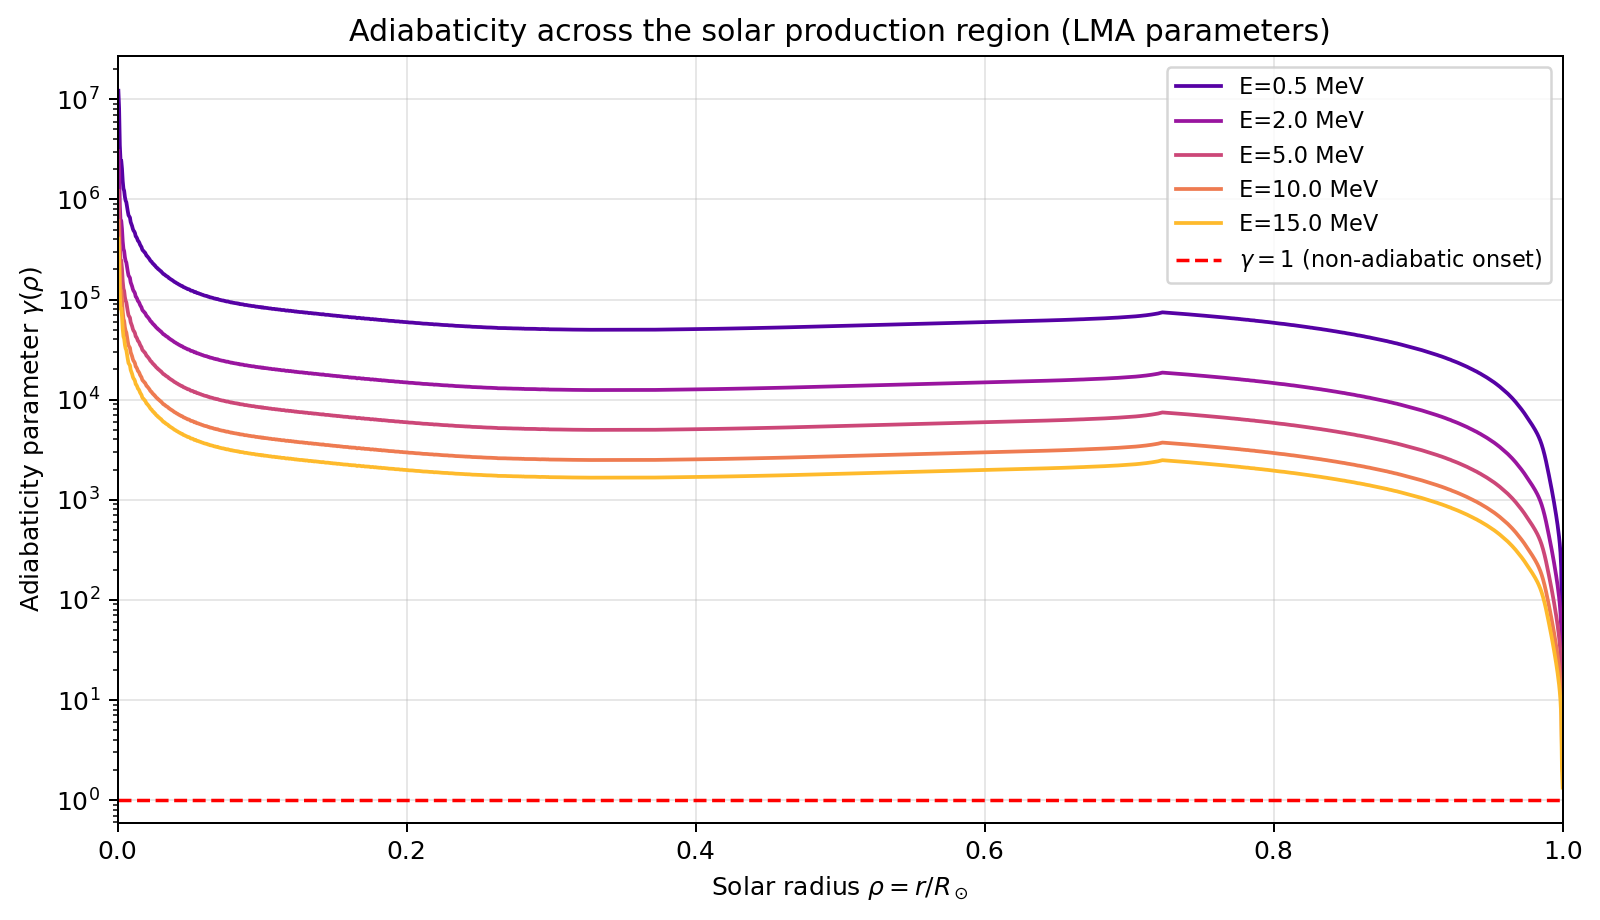
\includegraphics[width=0.75\textwidth]{figuras/resultados/sn3_fig5_adiabaticity_profile.png}
  \caption{Adiabaticity parameter \(\gamma(\rho)\) across the solar production region, for five representative energies, against the non-adiabatic onset \(\gamma=1\).}
  \label{fig:adiabaticity-profile}
\end{figure}

\subsubsection{CP violation}

\Cref{fig:cp-asymmetry-dune} shows the appearance probabilities \(P_{\mu e}\) and \(\bar P_{\mu e}\) at a long-baseline configuration (\(L=1300\,\mathrm{km}\)) for the NuFIT~5.2 best-fit CP phase, \(\delta_{\mathrm{CP}}=197^\circ\), and for maximal CP violation, \(\delta_{\mathrm{CP}}=-90^\circ\), together with the CP asymmetry \(A_{\mathrm{CP}}=P_{\mu e}-\bar P_{\mu e}\). The asymmetry is largest at low energy, where the genuinely CP-odd term dominates, and vanishes at the first oscillation node near \(E\sim1\,\mathrm{GeV}\), consistent with the expected \(L/E\) dependence.

\begin{figure}[htbp]
  \centering
  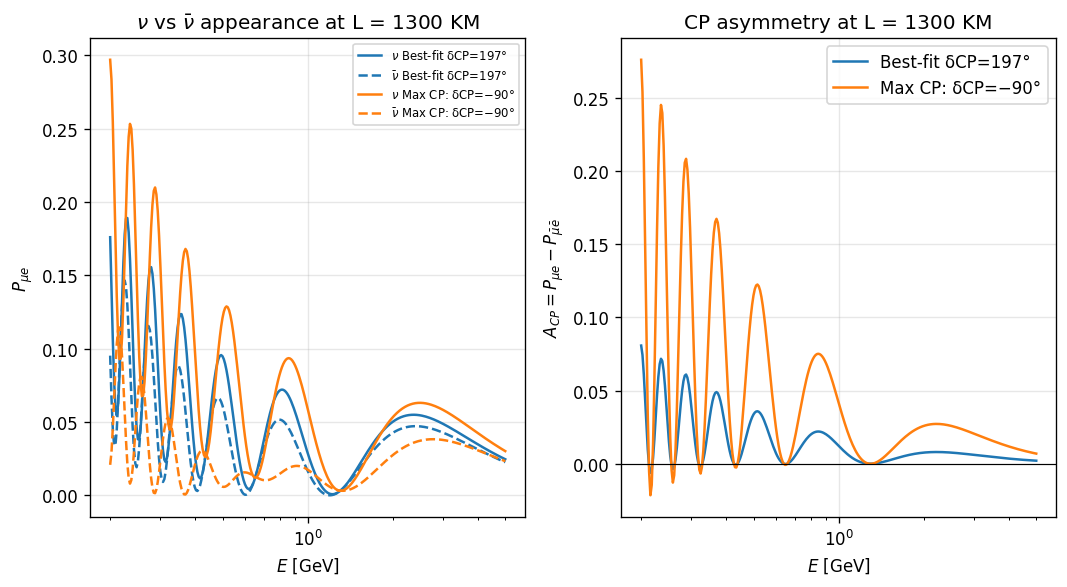
\includegraphics[width=0.9\textwidth]{figuras/resultados/vf3_fig32_1_cp_asymmetry.png}
  \caption{Appearance probabilities \(P_{\mu e}\) and \(\bar P_{\mu e}\) at a long-baseline configuration, \(L=1300\,\mathrm{km}\) (left) and the resulting CP asymmetry \(A_{\mathrm{CP}}\) (right), for the best-fit and maximal-CP-violation values of \(\delta_{\mathrm{CP}}\).}
  \label{fig:cp-asymmetry-dune}
\end{figure}

\subsubsection{Atmospheric neutrino oscillograms}

\Cref{fig:atm-oscillogram} shows the atmospheric \(\nu_\mu\) survival-probability oscillogram in the \((\cos\theta_z,E)\) plane, computed through the PREM Earth density profile \parencite{Dziewonski1981}. The characteristic vacuum oscillation dip is verified against the analytic first-minimum condition, \(1.267|\Delta m^2_{3\ell}|L/E=\pi/2\) \parencite{Ashie2004}, and against a set of benchmark observables summarised in \cref{tab:atmospheric-oscillogram}, spanning the atmospheric mass splitting and mixing angle, the vacuum \(L/E\) dip position, the multi-GeV up/down asymmetry, the energy of maximal mantle-crossing suppression, and the maximum appearance probability associated with the mantle MSW resonance.

\begin{figure}[htbp]
  \centering
  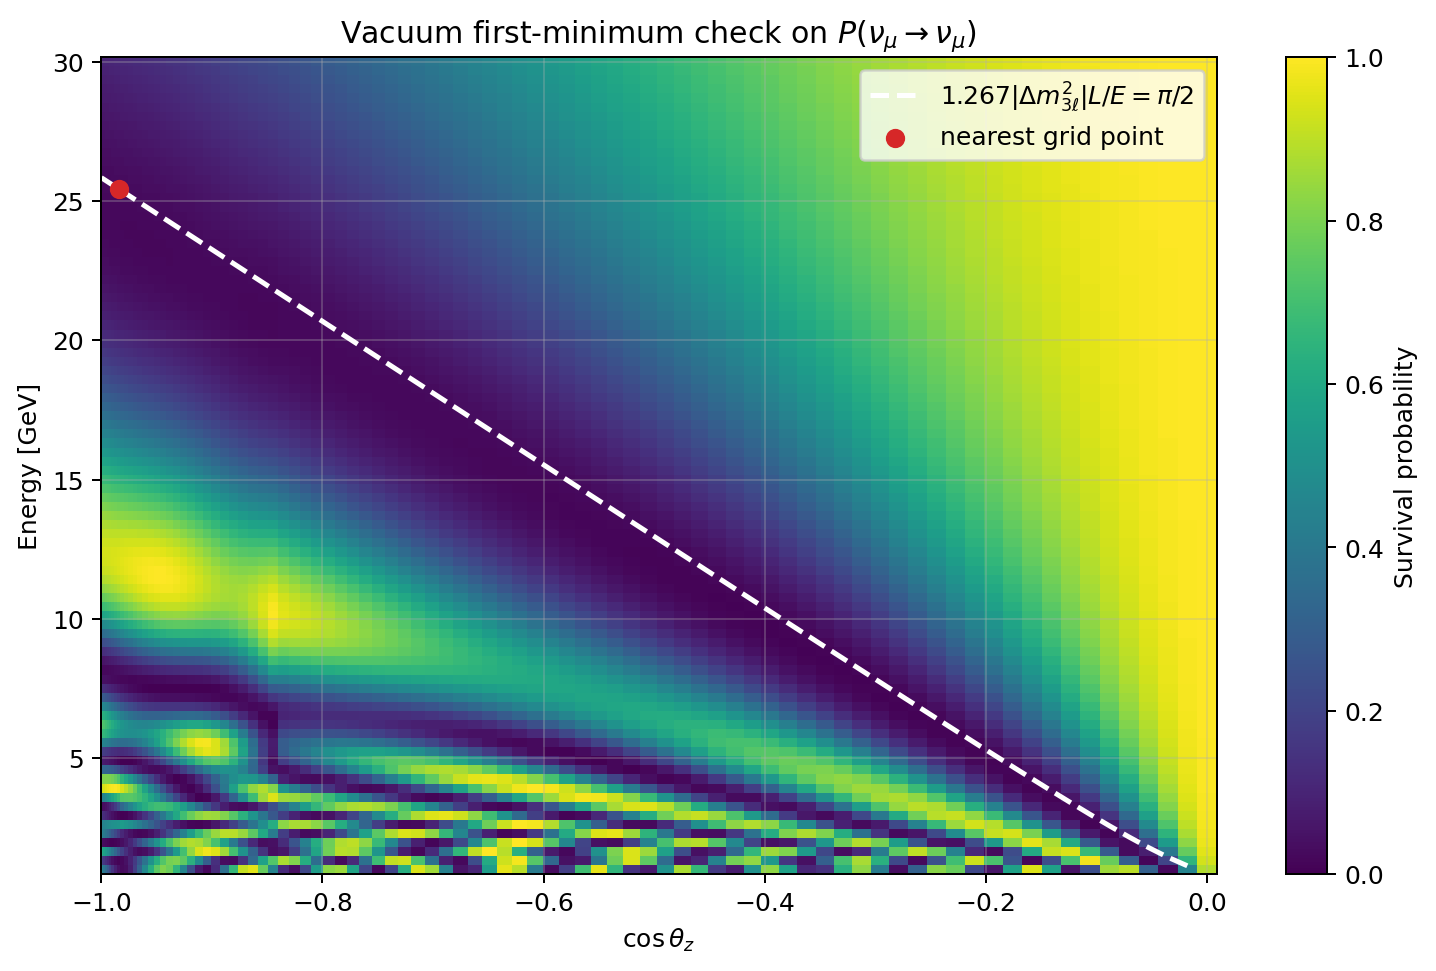
\includegraphics[width=0.75\textwidth]{figuras/resultados/oscillogram_numu_survival_first_minimum_check.png}
  \caption{Atmospheric \(P(\nu_\mu\to\nu_\mu)\) oscillogram in the \((\cos\theta_z,E)\) plane. The dashed line marks the analytic first vacuum-oscillation minimum, \(1.267|\Delta m^2_{3\ell}|L/E=\pi/2\); the red marker shows the nearest grid point.}
  \label{fig:atm-oscillogram}
\end{figure}

\begin{table}[htbp]
  \centering
  \footnotesize
  \caption{Benchmark observables reproduced from the atmospheric oscillogram, compared with published experimental results.}
  \label{tab:atmospheric-oscillogram}
  \begin{tabularx}{\textwidth}{Xlll}
    \toprule
    Observable & \texttt{tpeanuts} & Experiment & Reference \\
    \midrule
    \(|\Delta m^2_{3\ell}|\) [\(\mathrm{eV}^2\)] & \(2.511\times10^{-3}\) & \([1.9,3.0]\times10^{-3}\) & Wester et al. (2024), 90\% CL \\
    \(\sin^2(2\theta_{23})\) & 0.981 & \(>0.90\) & Wester et al. (2024), 90\% CL \\
    \(L/E\) [km/GeV] & 493.7 & \(\approx500\) & Ashie et al. (2004) \\
    \(A_\mu\) & \(-0.414\) & \(\approx-0.32\) & Fukuda et al. (1998) \parencite{SuperKamiokande1998} \\
    Max-suppression  [GeV] & 3.28 & 3--30~GeV range & Aartsen et al. (2013), DeepCore \\
    \(\max P(\nu_\mu\to\nu_e)\)  & 0.5904 & mantle MSW resonance & Aiello et al. (2024), KM3NeT/ORCA \\
    \bottomrule
  \end{tabularx}
\end{table}

\subsubsection{Earth matter tomography}

\Cref{fig:regen-derivative} shows the derivative of the electron-neutrino appearance probability with respect to the nadir angle, \(|dP_e/d\eta|\), which develops sharp, localised features precisely at the PREM shell boundaries \parencite{Dziewonski1981}, a pronounced spike at the core--mantle density jump and a regular oscillatory pattern for purely mantle-crossing trajectories, confirming that the propagation correctly resolves discontinuous density profiles, the basic requirement for neutrino tomography.

\begin{figure}[htbp]
  \centering
  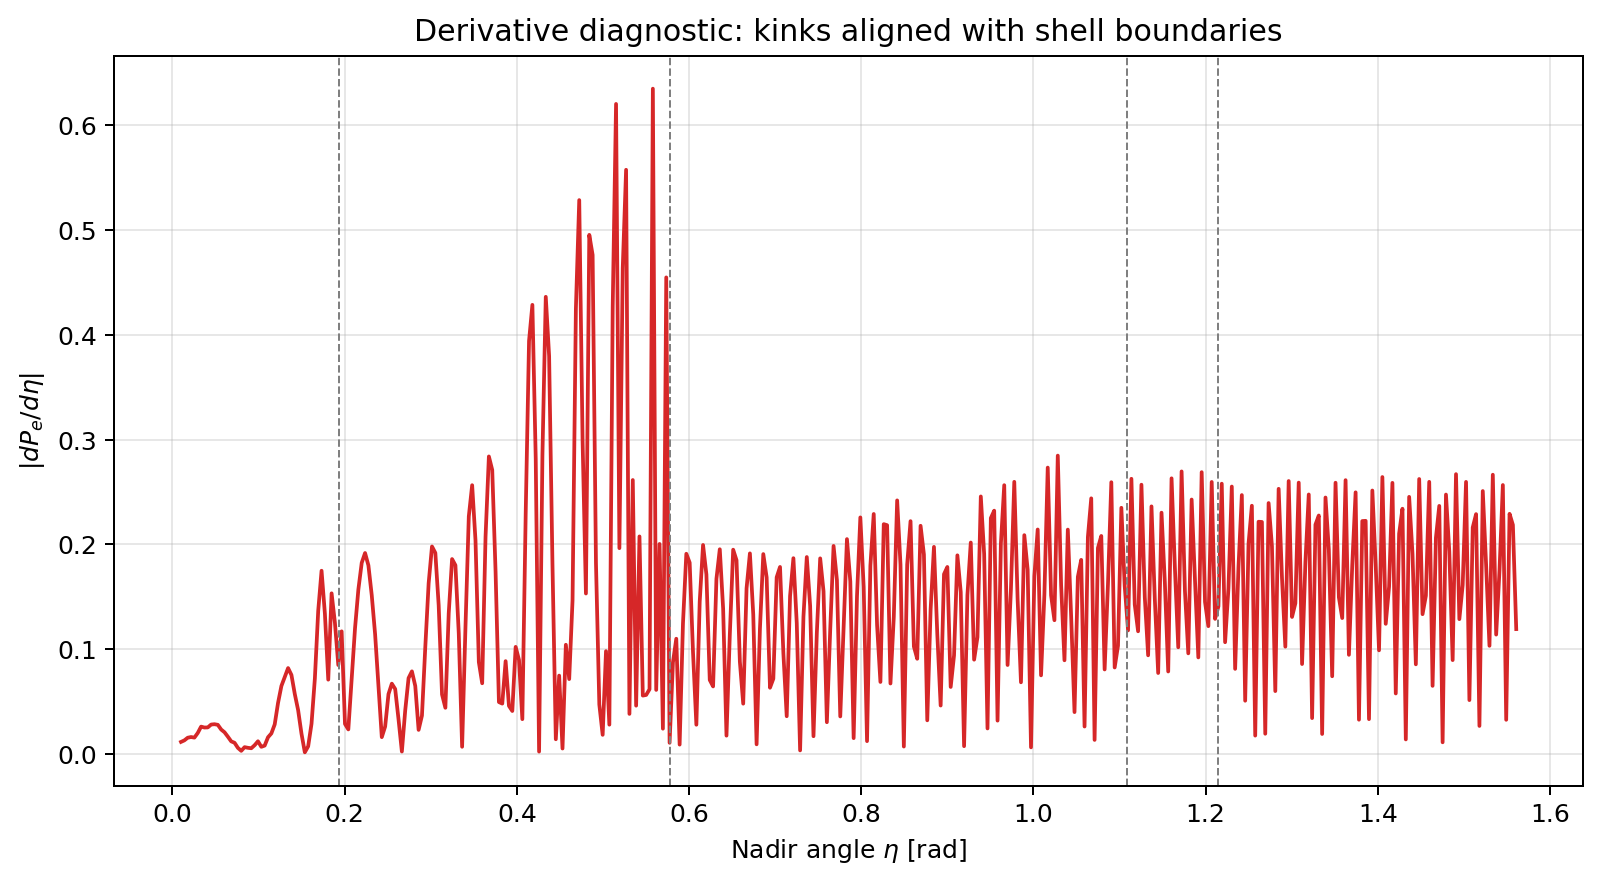
\includegraphics[width=0.75\textwidth]{figuras/resultados/regeneration_derivative.png}
  \caption{Derivative of the electron-neutrino appearance probability with respect to the nadir angle, \(|dP_e/d\eta|\); the dashed vertical lines mark the PREM shell boundaries.}
  \label{fig:regen-derivative}
\end{figure}

\subsection{BSM extensions}
\label{sec:bsm-results}

\subsubsection{NSI}

The propagation-NSI formalism introduced in \cref{sec:nsi-formalism} is validated by evaluating the solar \({}^8\mathrm{B}\) survival probability under several representative NSI presets drawn from the literature and from the projected sensitivity of upcoming experiments. \Cref{fig:nsi-presets} compares the Standard Model prediction (no NSI) against the diagonal bound of \textcite{Biggio2009}, an off-diagonal \(\varepsilon_{e\tau}=0.15\) coupling representative of DUNE's projected sensitivity, a combined \(\varepsilon_{ee}+\varepsilon_{e\tau}\) scenario representative of Hyper-Kamiokande, a purely off-diagonal \(\mu\tau\) coupling bounded by IceCube, and the global-fit values of \textcite{Esteban2018}. All presets converge to the same vacuum-averaged and adiabatic limits as the Standard Model at low and high energy, respectively, but distort the survival probability appreciably in the intermediate MSW transition region, by up to \(\sim2\) percentage points at \(E=10\,\mathrm{MeV}\); the largest distortions come from the global-fit and combined Hyper-K-like presets, while the purely \(\mu\tau\) off-diagonal coupling leaves \(P_{ee}\) exactly unchanged, since it does not couple directly to the electron-flavour survival probability at this order.

\begin{figure}[htbp]
  \centering
  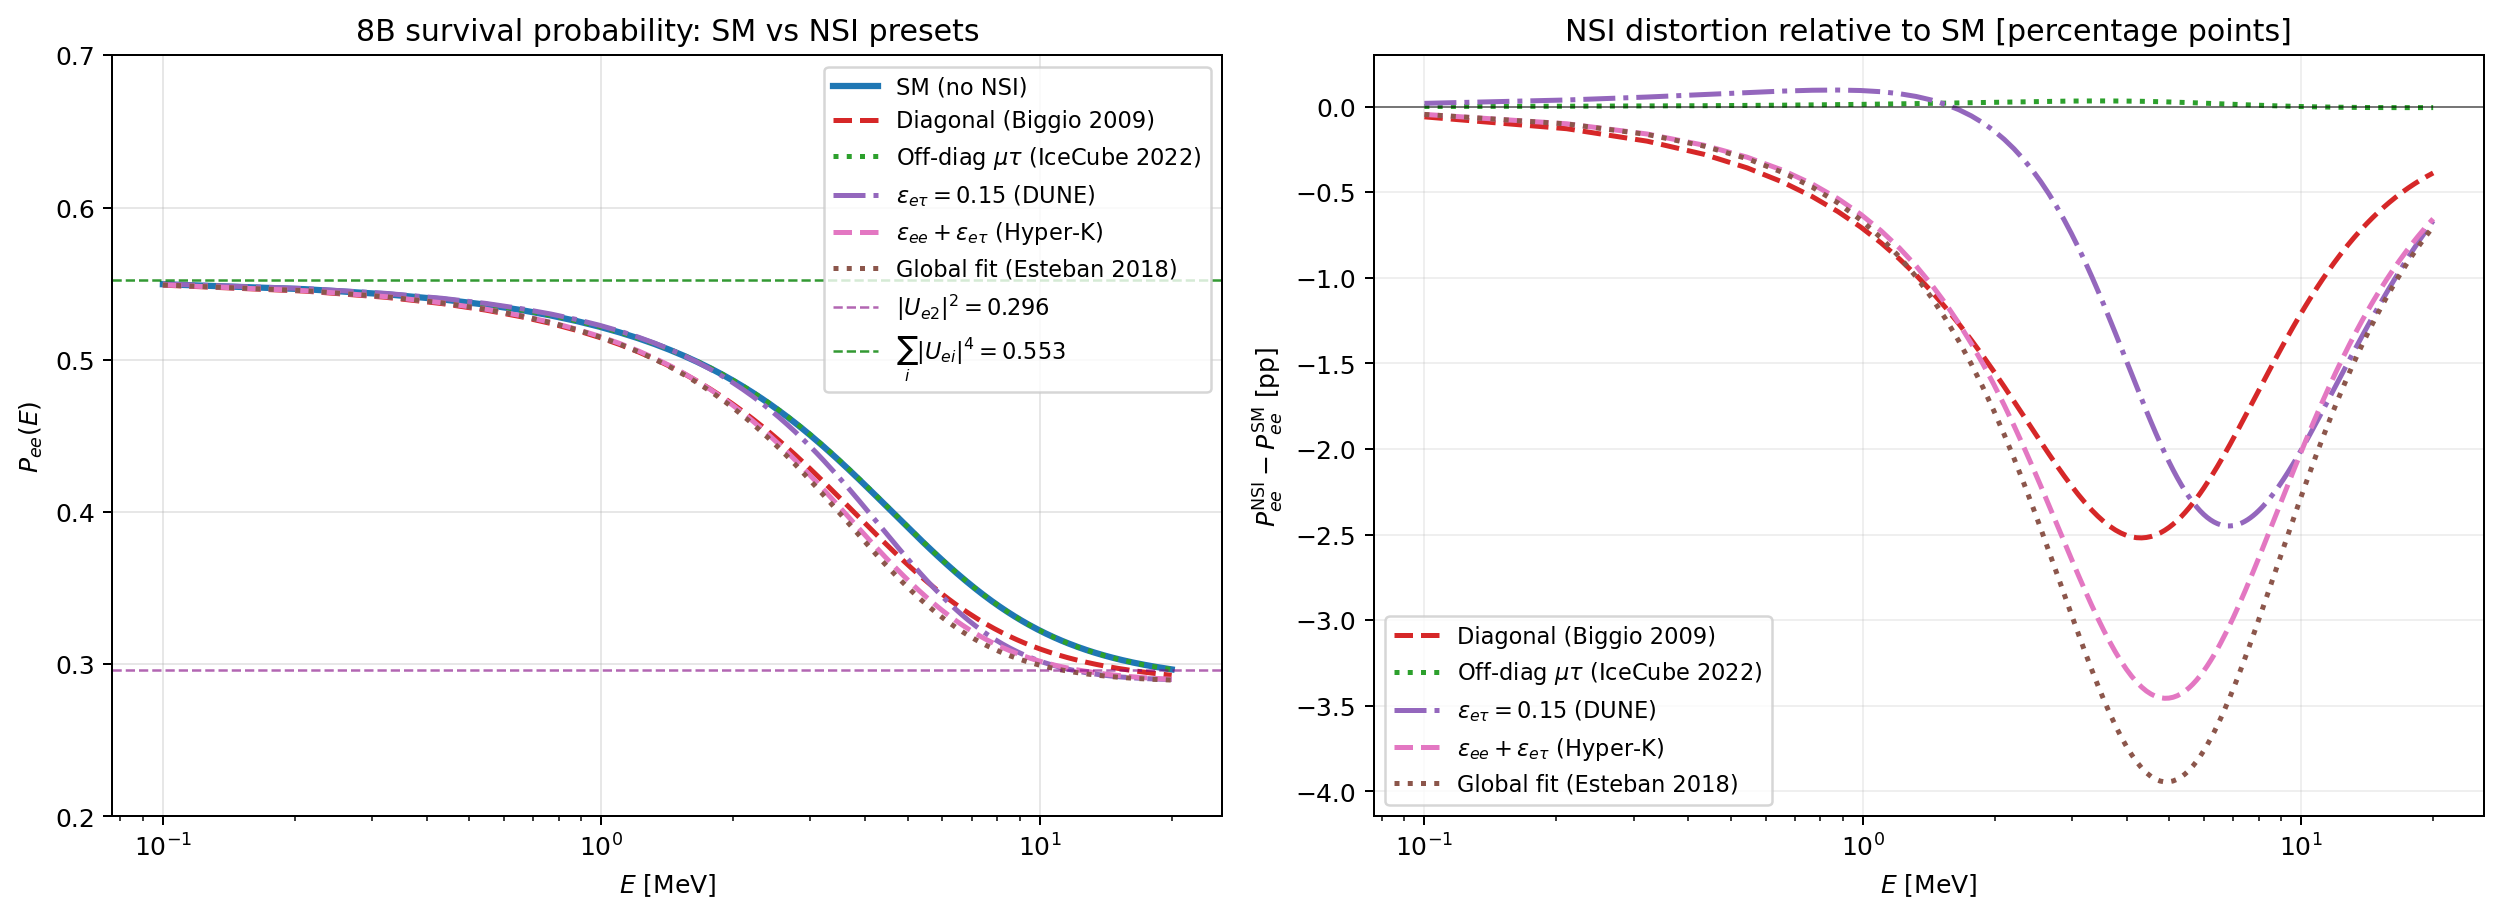
\includegraphics[width=\textwidth]{figuras/resultados/sn5_fig4_nsi_presets.png}
  \caption{\({}^8\mathrm{B}\) survival probability \(P_{ee}(E)\) under the Standard Model and several representative NSI presets (left), and the resulting distortion relative to the Standard Model, in percentage points (right).}
  \label{fig:nsi-presets}
\end{figure}

An independent scan of \(\varepsilon_{e\mu}\) and \(\varepsilon_{e\tau}\) over a representative range (\(-0.3\) to \(+0.3\)), with all other NSI parameters at zero, produces a clear, monotonic and oppositely signed distortion of the high-energy survival probability (\(E\gtrsim3\,\mathrm{MeV}\)) relative to the Standard Model for each coupling (\cref{fig:nsi-offdiag-scan}), confirming that the implementation correctly resolves both the sign and the magnitude dependence of each independent off-diagonal coupling.

\begin{figure}[htbp]
  \centering
  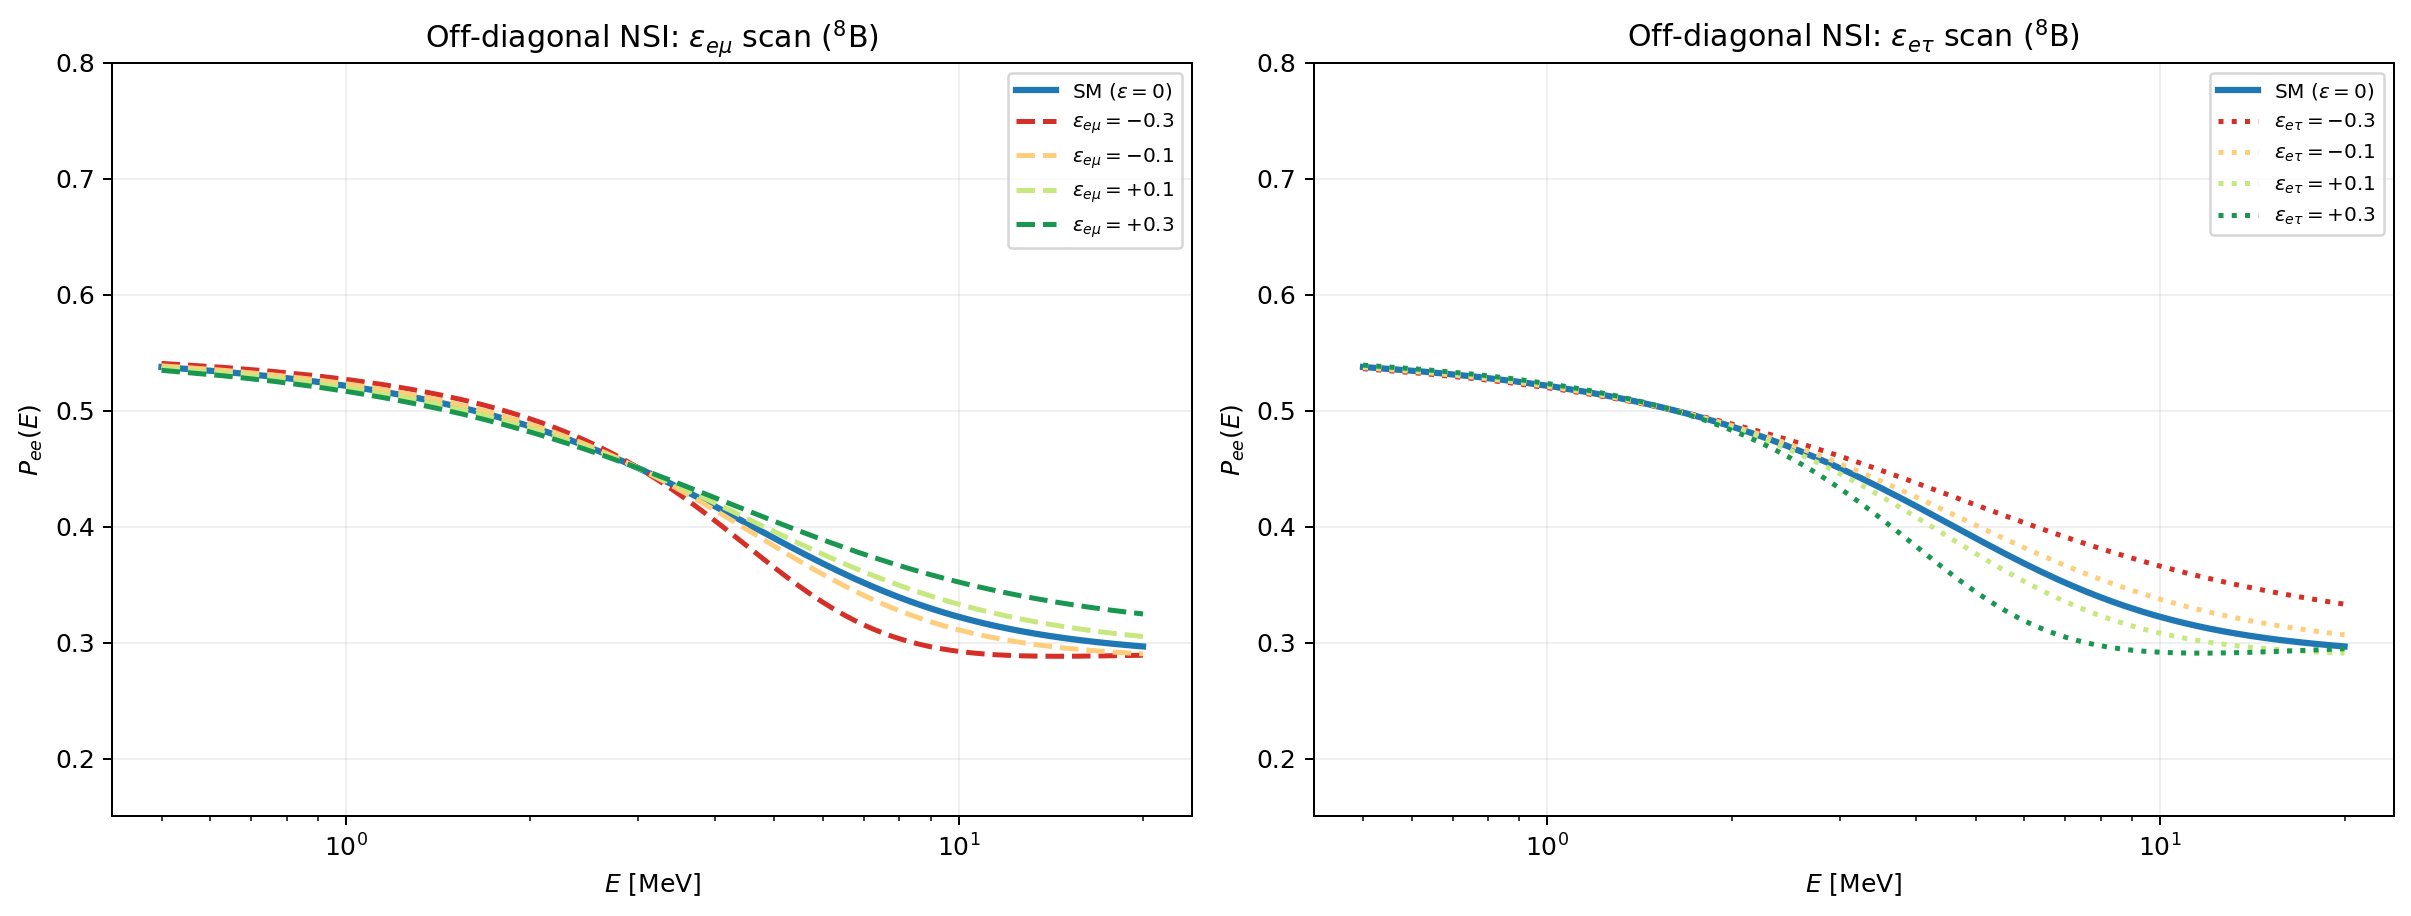
\includegraphics[width=0.85\textwidth]{figuras/resultados/sn5_fig6_offdiag_nsi.png}
  \caption{Distortion of the \({}^8\mathrm{B}\) survival probability \(P_{ee}(E)\) relative to the Standard Model, from independent scans of \(\varepsilon_{e\mu}\) and \(\varepsilon_{e\tau}\) over \(-0.3\) to \(+0.3\), with all other NSI parameters fixed to zero.}
  \label{fig:nsi-offdiag-scan}
\end{figure}

\subsubsection{Sterile neutrino}

The \(3+1\) sterile extension of \cref{sec:sterile-formalism} is validated against analytic expectations for three presets (a null-mixing reference, a Giunti (2017) global-fit-motivated best fit, and an IceCube (2020) benchmark), all propagated in vacuum. \Cref{tab:sterile-validation} summarises the confirmed, directly recorded results: the null-mixing preset recovers the Standard-Model limit to floating-point precision in the PMNS submatrix, the Hamiltonian and the vacuum probability; unitarity, \(\|U_4U_4^\dagger-I_4\|\), holds to \(\sim10^{-16}\) for all three presets; and, under the CC-only default (\cref{sec:sterile-formalism}, no neutron-density profile supplied), the sterile state is confirmed to receive no matter potential, both its row and column of the matter Hamiltonian vanishing identically. A dedicated CP-phase scan at LSND-like kinematics finds a maximal appearance asymmetry of only \(|A_{\mathrm{CP}}|\sim10^{-5}\), consistent with the standard result that appreciable \(3+1\) CP violation requires simultaneous sensitivity to two independent mass-squared splittings, not available at a single short baseline.

\begin{table}[htbp]
  \centering
  \footnotesize
  \caption{Confirmed \(3+1\) sterile-extension validation results.}
  \label{tab:sterile-validation}
  \begin{tabular}{@{}lr@{}}
    \toprule
    Check & Result \\
    \midrule
    SM-limit PMNS/Hamiltonian agreement (null mixing) & exact (\(0\) to printed precision) \\
    Unitarity \(\|U_4U_4^\dagger-I_4\|_F\) (three presets) & \(1.5\text{--}3.0\times10^{-16}\) \\
    Total vacuum probability \(\sum_\beta P_\beta\) & \(1.00000000\), max.\ dev.\ \(3.3\times10^{-16}\) \\
    Sterile row/column of matter Hamiltonian & exactly \(0\) \\
    Max.\ appearance CP asymmetry (LSND kinematics) & \(0.001\%\) at \(\delta_{14}=108.9^\circ\) \\
    \bottomrule
  \end{tabular}
\end{table}

The kinematic and phenomenological checks below are taken from companion validation notebooks. For \(\nu_e\), the two-flavour disappearance approximation is exact to \(10^{-14}\) in the idealised limit, its realistic-mixing deviation fully explained by the naive-versus-exact \(|U_{e4}|^2\) convention; for \(\nu_\mu\), a genuine residual of \(\mathcal O(10^{-2})\) survives even after this correction. Mapping the three presets onto reactor, Gallium, LSND/MiniBooNE and IceCube kinematics reproduces the well-known tension of the minimal \(3+1\) model: combining the reactor and IceCube disappearance bounds constrains the effective appearance amplitude to \(A_{e\mu}^{\mathrm{eff}}\lesssim0.003\), below the \(0.003\)--\(0.03\) required by LSND, a global tension \(>3\sigma\) consistent with the literature \parencite{Boser2020}. No inference notebook in the current implementation fits real short-baseline data with the sterile extension; this is left as future work.

\subsubsection{LMA-Dark degeneracy}

\Cref{fig:lma-dark-adn} reproduces the LMA-Dark degeneracy discussed in \cref{sec:validation-strategy}, comparing the day--night asymmetry predicted at fixed nadir angle (\(\eta=30^\circ\), \(1\,\mathrm{km}\) depth) under three scenarios: the standard LMA solution (\(\varepsilon_{ee}=0\)); a sign-flip demonstration in which only the Earth-matter NSI coupling is switched on (\(\varepsilon_{ee}=-2\)); and the full LMA-Dark approximation, obtained by simultaneously transforming \(\theta_{12}\to\pi/2-\theta_{12}\) and \(\varepsilon_{ee}\to-(2+\varepsilon_{ee})\). The standard-LMA solution gives \(A_{\mathrm{DN}}\approx+4.8\%\), broadly consistent with the Super-Kamiokande measurement \(A_{\mathrm{DN}}=(3.3\pm1.0)\%\) \parencite{SuperKamiokande2016}; switching on only the Earth-matter NSI coupling flips the sign, \(A_{\mathrm{DN}}\approx-1.6\%\); and the full LMA-Dark approximation gives \(A_{\mathrm{DN}}\approx-2.9\%\), the wrong sign relative to the Super-Kamiokande band and disfavoured by it at the \(\sim3\sigma\) level. Unlike the vacuum mixing angle alone, which is degenerate under the LMA-Dark transformation, the Earth-matter day--night asymmetry breaks the degeneracy at this coupling strength, illustrating why complementary observables beyond the vacuum survival probability are needed to resolve it in general.

% TODO: bsm3_fig5_adn.png below still reflects the pre-2026-07-16 NSI/sterile bug
% fixed in commit 89ce6cf (core.BSM pytest suite). Regenerate by re-running
% notebooks/physics/experimental_results/BSM/NSI2_lma_dark.ipynb; the corrected
% numbers already quoted above (A_DN ~ +4.8% / -1.6% / -2.9%) come from that
% notebook's current cached output.
\begin{figure}[htbp]
  \centering
  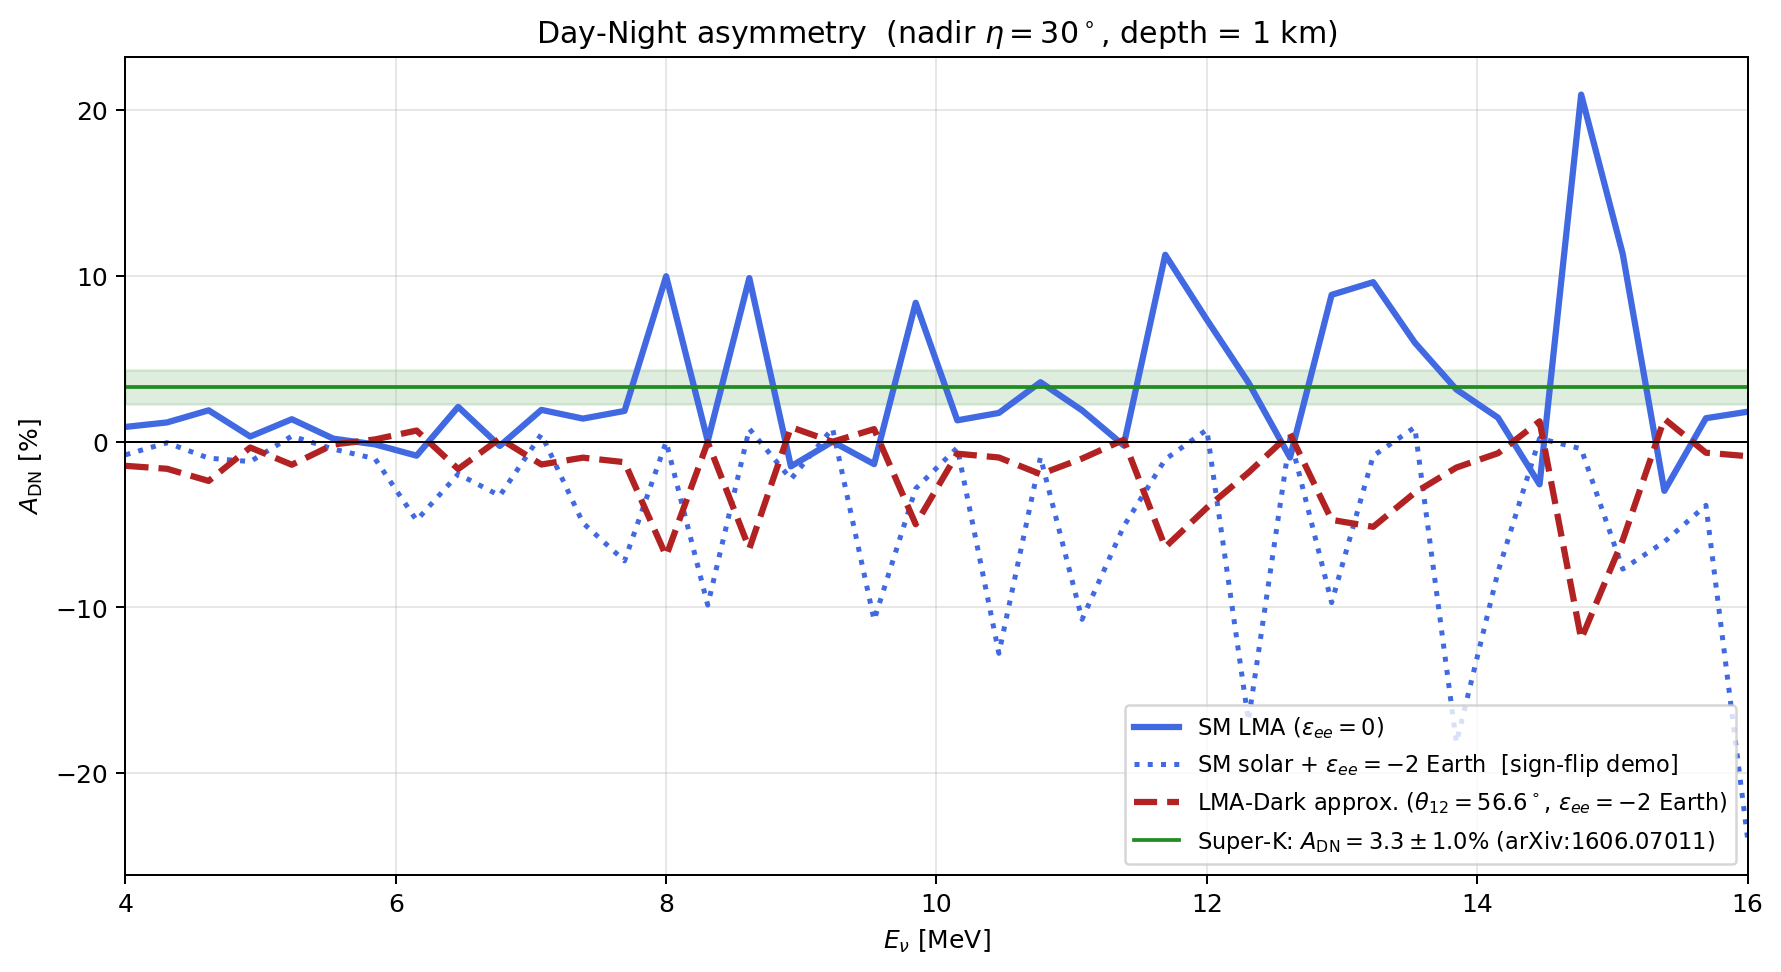
\includegraphics[width=0.85\textwidth]{figuras/resultados/bsm3_fig5_adn.png}
  \caption{Day--night asymmetry versus energy at fixed nadir angle (\(\eta=30^\circ\), \(1\,\mathrm{km}\) depth), comparing the standard LMA solution, a sign-flip demonstration with an Earth-only NSI coupling, and the full LMA-Dark approximation, against the Super-Kamiokande measurement \parencite{SuperKamiokande2016}.}
  \label{fig:lma-dark-adn}
\end{figure}

\subsection{Inference with real experimental data}
\label{sec:inference-real-data}

\subsubsection{Detector-level case study: Daya Bay}
\label{sec:dayabay-case-study}

The detector and inference layers of \cref{sec:detector-layer,sec:inference-layer} are validated end to end against the real, published Daya Bay reactor-antineutrino data set: 8 antineutrino detectors (ADs) at three experimental halls, 6 reactor cores, and the 8-AD-period inverse-beta-decay (IBD) prompt-energy spectra, following the methodology of \cref{sec:detector-validation-methodology}.

\begin{table}[htbp]
  \centering
  \footnotesize
  \caption{Daya Bay closure test: predicted vs.\ observed IBD counts at Daya Bay's own published \((\theta_{13},\Delta m^2_{31})\), no fit.}
  \label{tab:dayabay-closure}
  \begin{tabular}{@{}lrrr@{}}
    \toprule
     & Predicted & Observed & Ratio \\
    \midrule
    Total (8 detectors) & 3\,705\,407 & 3\,114\,934 & 1.190 \\
    \bottomrule
  \end{tabular}
\end{table}

\Cref{tab:dayabay-closure} shows the closure test: evaluated at Daya Bay's own published oscillation parameters with no free normalisation, the forward model over-predicts the observed rate by \(\approx19\%\), remarkably uniformly across all 8 detectors. A dedicated normalisation audit traced this gap through every stage of the absolute-rate chain, target mass, efficiency, cross section (independently validated to \(\sim1\%\) against Vogel \& Beacom's own quoted coefficient), and the Huber--Mueller yield, identifying and quantifying its dominant sources, with no unit-conversion error found at any traced stage (a compensating error elsewhere in the chain would not be excluded by this audit alone): part of the gap is the well-known, independently measured Reactor Antineutrino Anomaly (\(\sim5\)--\(6\%\), measured/predicted flux ratio \(0.946\pm0.020\) \parencite{An2017DayaBayFluxSpectrum}), and the remainder is consistent with the correlated normalisation systematics Daya Bay's own combined analysis also carries, precisely why a free \(\nu_{\mathrm{norm}}\) nuisance is included in the fits below rather than fixed to 1.

Comparing the predicted and observed prompt-energy spectra for one near-hall and one far-hall detector shows that both share the same IBD-kinematics-driven shape, with the far-hall spectrum visibly suppressed relative to its no-oscillation expectation, the qualitative signature the measurement is built on. Fitting the full 8-detector, 208-bin spectral shape jointly over \((\theta_{13},\Delta m^2_{31},\nu_{\mathrm{norm}})\) was attempted with increasingly rich nuisance freedom (background-rate and energy-scale-non-linearity pulls); none of the three attempts converges to a physical point, and adding energy-scale pulls makes the fit worse, \(\hat\theta_{13}\) collapsing to \(0^\circ\), a genuine degeneracy between the oscillation deficit and uncorrelated energy-scale freedom rather than a bug. This is reported as a diagnosed limitation: it demonstrates why real reactor experiments build a full correlated systematic covariance rather than a handful of independent nuisances once sub-percent shape residuals dominate the statistical error.

Two simpler observables, by contrast, converge robustly. Integrating each detector's spectrum to a single rate and fitting \((\theta_{13},\nu_{\mathrm{norm}})\) with \(\Delta m^2_{31}\) fixed gives \(\hat\theta_{13}=8.389^\circ\pm0.139^\circ\) (\(\sin^22\theta_{13}=0.08332\)), \(-2.66\%\) relative to Daya Bay's published \(0.08560\) (\(-0.85\sigma\)). The near/far ratio fit, mirroring Daya Bay's own 2012 discovery strategy \parencite{An2012DayaBayDiscovery}, is the only strategy with genuine joint sensitivity to both parameters, and is the headline result of this case study:

\begin{table}[htbp]
  \centering
  \footnotesize
  \caption{Daya Bay near/far ratio fit vs.\ Daya Bay's own published best fit and NuFIT~6.0 \parencite{EstebanNuFit2024}.}
  \label{tab:dayabay-summary}
  \begin{tabular}{@{}lrrr@{}}
    \toprule
    Quantity & \texttt{tpeanuts} (near/far) & Daya Bay published & NuFIT 6.0 \\
    \midrule
    \(\sin^22\theta_{13}\) & 0.08442 & 0.0856 \parencite{An2023DayaBayPrecision} & 0.0878 \\
    \(\theta_{13}\) [deg] & \(8.445\pm0.134\) & 8.506 & 8.62 \\
    \(\Delta m^2_{31}\) [\(10^{-3}\)eV\(^2\)] & \(2.478\pm0.055\) & 2.528 & 2.511 \\
    \bottomrule
  \end{tabular}
\end{table}

\begin{figure}[htbp]
  \centering
  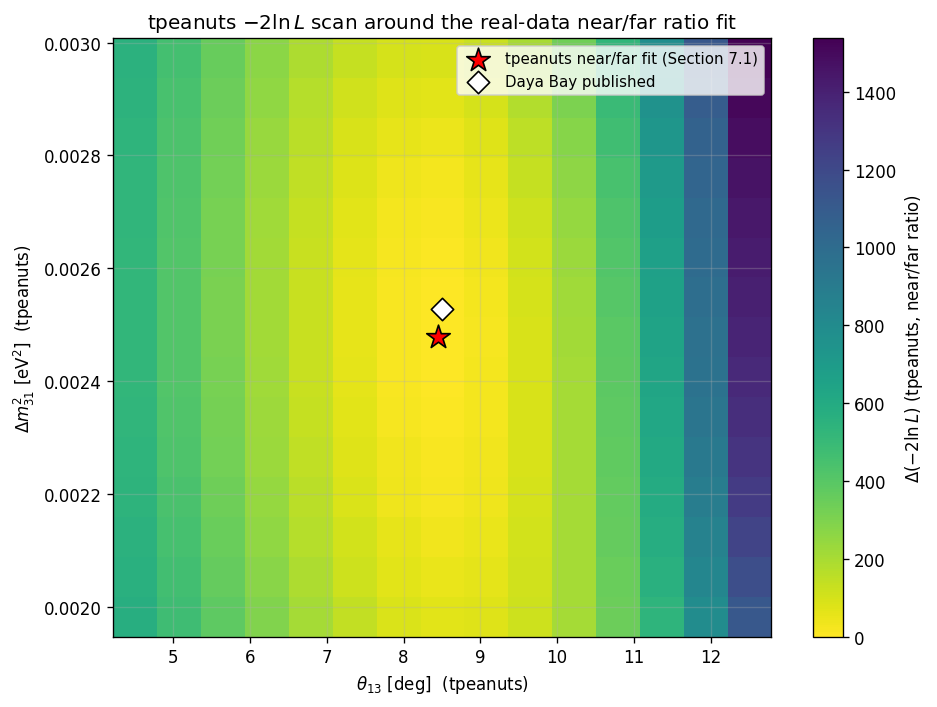
\includegraphics[width=0.75\textwidth]{figuras/resultados/dayabay_fig7_nearfar_scan.png}
  \caption{\texttt{tpeanuts} \(-2\ln L\) scan around the real-data near/far ratio fit, in the \((\theta_{13},\Delta m^2_{31})\) plane, compared with Daya Bay's own published best fit (\cref{sec:supplementary-material}).}
  \label{fig:dayabay-nearfar-scan}
\end{figure}

A 2-D \(-2\ln L\) scan over \((\theta_{13},\Delta m^2_{31})\), shown in \cref{fig:dayabay-nearfar-scan}, confirms that the fitted point and Daya Bay's own published point sit well inside the same low-\(\Delta(-2\ln L)\) region. As \cref{tab:dayabay-summary} shows, the near/far fit recovers both \(\sin^22\theta_{13}\) and \(\Delta m^2_{31}\) jointly, within \(1\)--\(2\%\) of Daya Bay's own published values and comfortably inside NuFIT's global-fit range, using \texttt{tpeanuts}'s own real multi-reactor flux, order-\(1/M\) cross section and IAV+LSNL+Gaussian detector response, not a synthetic data set. This is the clearest demonstration that the detector and inference layers, built on top of the validated oscillation engine of \cref{sec:validation-strategy}, extend \texttt{tpeanuts} from fast forward simulation to genuine gradient-based analysis of real experimental data.

\subsubsection{Other detector-inference applications}
\label{sec:other-experiments}

The same detector and inference layers are applied to four further real experiments (\cref{tab:detector-experiments}), documented in full, with their own validation figures, in the specialised documents referenced in \cref{sec:supplementary-material}:

\begin{itemize}
  \item \textbf{IceCube DeepCore}: a 4-parameter Poisson fit to 9 years of golden atmospheric-event data recovers \(\theta_{23}=45.42^\circ\pm1.85^\circ\) and \(\Delta m^2_{3l}=(2.395\pm0.039)\times10^{-3}\,\mathrm{eV}^2\), a \(-0.05\sigma\) pull on \(\sin^2\theta_{23}\) relative to the collaboration's published best fit; a dedicated audit of the fitted muon-background normalisation (\(16\%\) above the published value) rules out an Earth-matter-unitarity origin (a \(0.002\%\) effect) and instead traces most of the gap to fixed detector-systematics hypersurfaces (up to \(+12\%\) for the \(\nu_\tau\)-CC channel) not yet freed as nuisance parameters.
  \item \textbf{SNO phase~II}: a fit to the full 391-day, 38-observable salt-phase data set, using the published statistical covariance plus a reconstructed systematic covariance that does not yet include the NC channel's dedicated systematics, converges to \(\theta_{12}=35.28^\circ\pm1.61^\circ\), \(\Delta m^2_{21}=(6.10\pm34{,}900)\times10^{-5}\,\mathrm{eV}^2\); \(\theta_{12}\) sits inside SNO's own SNO-only \(1\sigma\) range, while the reported \(\Delta m^2_{21}\) uncertainty illustrates the Laplace approximation breaking down once the highly correlated reconstructed covariance is included, exactly why the likelihood-scan machinery of \cref{sec:inference-layer} exists.
  \item \textbf{Borexino}: the elastic-scattering event-rate chain (target, response, cross section) is implemented and unit-tested against the real Nature~2018 low-energy spectrum \parencite{Agostini2018Borexino}, but its background model is currently a documented placeholder, so no fit to real data is yet reported.
  \item \textbf{SNO phase~I}: a day/night spectral fit to real published data converges robustly to \(\theta_{12}=34.333^\circ\pm0.665^\circ\), a \(0.86\sigma\) pull relative to NuFIT~6.1.
\end{itemize}

\subsection{Public repository and supplementary material}
\label{sec:supplementary-material}

The full source code of \texttt{tpeanuts}, together with the notebooks used for validation, analysis and benchmarking, is publicly available in the following GitHub repository:

\begin{center}
  \url{https://github.com/juanramondiaz/tpeanuts}
\end{center}

The repository is organised so that the physical modules are kept separate from the notebooks that exercise them; \texttt{notebooks/} is the main entry point for reviewing results and reproducing figures (\cref{tab:notebook-tree}).

\begin{table}[htbp]
  \centering
  \footnotesize
  \caption{Notebook directory tree (paths relative to \texttt{notebooks/} in the repository above).}
  \label{tab:notebook-tree}
  \begin{tabularx}{\textwidth}{XX}
    \toprule
    Path & Contents \\
    \midrule
    \texttt{physics/\allowbreak simulation/\allowbreak\{vacuum,\allowbreak solar,\allowbreak earth,\allowbreak atmosphere\}} & Fundamentals, production/exposure profiles and differential-flux analysis per medium. \\
    \texttt{physics/\allowbreak experimental\_results/\allowbreak\{vacuum,\allowbreak solarneutrino,\allowbreak atmosphericneutrino,\allowbreak BSM\}} & Reproduction of the physical signatures of \cref{sec:experimental-reproduction-results} and \cref{tab:sterile-validation}. \\
    \texttt{validation/\allowbreak\{nusquids,\allowbreak legacy\}} & Cross-validation against \texttt{nuSQuIDS} and bit-level validation against legacy PEANUTS. \\
    \texttt{inference/} & Detector-level closure tests and gradient-based fits to real data (Borexino, SNO, Daya Bay, IceCube DeepCore, SNO~II; \cref{sec:dayabay-case-study,sec:other-experiments}). \\
    \texttt{benchmark/} & Performance comparison against PEANUTS and \texttt{nuSQuIDS}. \\
    \texttt{external/\allowbreak\{corsika,\allowbreak nusquids,\allowbreak prem,\allowbreak zenodo,\allowbreak reactor/\allowbreak dayabay\}} & CORSIKA generation and exploratory/data-retrieval notebooks for external inputs. \\
    \bottomrule
  \end{tabularx}
\end{table}

Full architectural and physics detail beyond the scope of this thesis, module by module, is documented separately in five companion \LaTeX{} documents shipped alongside the code (\texttt{documentation/}), each with its own figures and, for the inference documents, its own real-data results: \texttt{guide} (\texttt{core}, \texttt{medium}, \texttt{pipeline}, \texttt{detector.common/interaction/borexino}); \texttt{BSM\_NSI} and \texttt{BSM\_sterile} (theory, implementation and notebook results for each BSM extension, \cref{tab:sterile-validation}); and \texttt{inference\_dayabay}, \texttt{inference\_icecube}, \texttt{inference\_sno\_ii} (full detector implementation and real-data results underlying \cref{sec:dayabay-case-study,sec:other-experiments}).
